\documentclass[final]{usydphysthesis}
% \documentclass[draft]{usydphysthesis}

% Figures directory
\graphicspath{{figures/}}

% Define new float enviornment
\DeclareCaptionType{algorithm}[Algorithm][List of Algorithms]

% biblatex loaded by cls file
\addbibresource{main.bib}

% Let tensors be math bold
\let\ten\mathbf

\NewDocumentCommand{\bao}{}{\textsc{bao}}
\NewDocumentCommand{\cmb}{}{\textsc{cmb}}
\NewDocumentCommand{\matlab}{}{\textsc{matlab}}
\NewDocumentCommand{\mcmc}{}{\textsc{mcmc}}
\NewDocumentCommand{\snap}{}{\textsc{snap}}

% Shorthand for rho crit
\NewDocumentCommand{\rhoc}{}
{\ensuremath{
    \rho_{\mathrm{crit}}
}}

% mathrm d for dx
\NewDocumentCommand{\dd}{m}{
    \mathop{}\!\mathrm{d}#1
}

% Shortcut for p(a) and p(A|B)
\NewDocumentCommand{\prob}{m o}
{\ensuremath{
    \operatorname{p}
    \IfValueTF{#2}
      {
        \!\left(
          #1
          \middle|
          #2
        \right)
      }
      {
        \!\left(
          #1
        \right)
      }
}}

% Automatic figure labels
\ExplSyntaxOn
\NewDocumentCommand{\staticfigure}{ O{\textwidth} m m }{%
  \begin{center}
    \includegraphics[width=#1]{#2}
    \captionof{figure}{#3}%
    \__fvbb_label_from_filename:n {#2}%
  \end{center}
}

% For use in subfigures
\NewDocumentCommand{\staticsubfigure}{ O{0.48\textwidth} m m }{%
  \begin{subfigure}[t]{#1}
  \begin{center}
    \includegraphics[width=\linewidth]{#2}
    \caption{#3}
    \__fvbb_label_from_filename:n {#2}
  \end{center}
  \end{subfigure}%
}

% Get lbel from file basename
\cs_new_protected:Npn \__fvbb_label_from_filename:n #1
  {
    % strip path
    \tl_set:Nn \l_tmpa_tl {#1}
    \regex_replace_once:nnN {^.*/} {} \l_tmpa_tl
    % strip extension
    \regex_replace_once:nnN {\.[^.]+$} {} \l_tmpa_tl
    % create label
    \label{fig:\tl_use:N \l_tmpa_tl}
}
\ExplSyntaxOff
  
% Maketitle
\title{Bayesian Analysis of Type Ia Supernovae as Dark Energy Probes}
\subtitle{} % optional

\author{Francesca von Braun-Bates}

\thesistype{A thesis}
\degree{Bachelor of Science (Honours)}
\department{School of Physics}
\university{The University of Sydney}
\date{December 2010}

% ------------------------------------------------------

\begin{document}
\frontmatter

\maketitle

   Dark energy and gravity are equally important in determining the large-scale geometry and evolution of the universe. This evolution can be computationally modelled using the Friedmann ODEs obtained from the general relativistic Friedmann-Robertson-Lemaitre-Walker metric tensor.  Under the assumption of a spatially flat universe with its only contents being matter and a time-varying dark energy, the parameters in the Friedmann equations reduce to the Hubble constant, the cosmological matter density, the two-parameter dark energy equation of state and a matter-dark energy interaction parameter. 

   I demonstrate the use of Bayesian inference to estimate values for these cosmological parameters (with the excpetion of the Hubble constant, as this cannot be extracted from the data). 

   The parameters are related to observations by redshift-distance relations. I focus on the luminosity distance, which can be measured using Type Ia supernovae. The data used is a selection of three recent SNe compilations and five artificially generated sets: three based on these compilations to see how the parameter uncertainty scales with error and two projected data sets based upon the upcoming Supernova Acceleration Probe. I use the Metropolis-Hastings algorithm, an example of Markov chain Monte Carlo methods, to generate the posterior probability distributions for models with one and two free parameters (although the code I wrote can be used for up to $n$ parameters). Credible regions can be generated for the parameter space from the posterior distributions. 

   I conclude that the one-parameter distributions show that the currently accepted ”concordance cosmology” is a plausible approximation to the parameters, although differences in the light curve fitters which were used to calibrate the data prevent a more decisive estimation. The two-parameter models exhibit a wide range of degeneracies which need to be resolved by combining the supernova-derived credible regions with those from the cosmic microwave background and baryon acoustic oscillations.



\tableofcontents
\listoffigures
\listoftables

\mainmatter

% chapters/intro.tex
\chapter{Introduction}
\label{ch:introduction}

% ---------- Chapter 1: Introduction ----------

\begin{figure}
\centering

\begin{subfigure}{0.45\textwidth}
  \centering
  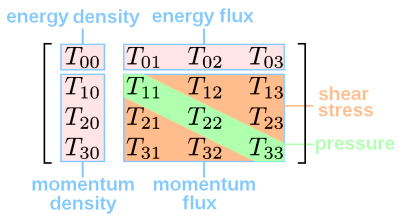
\includegraphics[width=.8\textwidth]{figures/chapter1/fig1.1}
  \caption{The general stress-energy tensor.}
  \label{fig:stress-energy-general}
\end{subfigure}
\hfill
\begin{subfigure}{0.45\textwidth}
  \centering
  \[
  \begin{pmatrix}
    c^{2} \rho{} & 0 & 0 & 0 \\
    0 & p & 0 & 0 \\  
    0 & 0 & p & 0\\
    0 & 0 & 0 & p
  \end{pmatrix}
  \]
  \caption{Perfect fluid case.}
  \label{fig:stress-energy-perfect}
\end{subfigure}
\caption{The stress-energy-momentum tensor for the general case and a perfect fluid.}
\label{fig:1.1}
\end{figure}

\begin{figure}
\centering
    \staticfigure[0.75\textwidth]{figures/chapter1/fig1.2.png}{SNe classes based on spectroscopy, with well-known examples of each class. Type Ia are thought to be the result of thermonuclear explosions, whereas all other types are caused by core collapse in massive stars. Type IIb are a crossover class, initially appearing as Type II but evolving into Type Ib/c. Image credit: Fig. 1 in \cite{Leibundgut2008}.}
\end{figure}

\begin{figure}
\centering
    \staticfigure[0.75\textwidth]{figures/chapter1/figure1.3.jpeg}{Type Ia SNe formation. This shows a singly-degenerate supernova, in which the white dwarf accretes matter from a companion star. The dwarf eventually reaches the Chandrasekhar limit, at which point its mass is too great for the dwarf to remain stable and it implodes.  Image credit: Fig. 10 of \cite{Matteucci2008}.}
\end{figure}

% CHAPTER TEXT  ----------------------------------------

Dark energy is one of the most important and least understood components of the universe. Its first introduction was the inclusion of the cosmological constant in Einstein’s equation of general relativity. Ironically, astronomical observations which indicated an expanding universe caused firstly the removal of the constant \cite{Harrison1993} and then its reintroduction \cite{Hobson2006}. Re-interpretation of the cosmological constant as a form of energy (rather than an independent scalar parameter) lead to the proposal of a broader class of ”anti-gravity fluids” which are now known as dark energy \cite{Hobson2006}. Attempts to differentiate between competing dark energy models have lead cosmologists to widen their search for evidence of expansion: the first hint of dark energy came from studies of Type Ia supernovae \cite{Leibundgut2008} but now studies (e.g. \cite{Amanullah2010,LewisBridle2002}) combine data from a variety of sources including supernovae \cite{Hicken2009,Riess2007,Kowalski2008}, the cosmic microwave background (\cmb{}), \cite{LewisBridle2002} and baryon acoustic oscillations (BAO) \cite{Komatsu2010}. 

This thesis aims to use Bayesian analysis to investigate the usefulness of Type Ia supernovae as dark energy probes. Markov Chain Monte Carlo methods are applied to determine constraints from Ia SNe on four cosmological parameters: the fractional density of matter, the (two-parameter) dark energy equation of state and the interaction constant. (The Hubble constant is included as an additional free parameter.) The data sets used in the \mcmc{} method come from three sources: observational data calibrated and processed by supernova survey groups, the same data sets with reduced errors (to investigate how uncertainties in the cosmological parameters scale with uncertainties in the observational data) and two projected sets based upon a recently-proposed, space-based survey. There is ample scope for further work in observational, computational and theoretical areas, a brief discussion of which concludes the thesis.

\section{Cosmological background}
\label{sec:cosmological-background}

The framework of modern cosmology depends upon the cosmological principle. The is an indemonstrable assumption that at a given time the universe is, apart from local irregularities, the same at all points in space. We can only prove directly that the universe is isotropic about our location. Therefore, rather than proving that the universe is isotropic and homogeneous everywhere, we must show that homogeneity is likely by demonstrating the gross improbability of a ”preferred location” which alone is isotropic \cite{Harrison1993}. Once homogeneity is established, the cosmological principle follows directly: the universe is everywhere (and everywhen) homogeneous and isotropic. Only once we have made this assumption can we propose that the laws of physics are the same at all times and places. We can now use the entire observable universe as a laboratory: if a theory can be proven false by a distant event, then it must also be false everywhere else.\footnote{This does not discard the usefulness of a failed theory as an approximation is some cases e.g. Newtonian gravity.} Conversely we can also apply physical laws to any point in the Universe. The assumption of the cosmological principle permits the application of physics on the largest scales\footnote{\cite{Hartle2003} quantifies large scale as more than hundreds of Mpc.} provided that we impose homogeneity and isotropy on the universe.

\section{General Relativity}
\label{sec:1.2}

The Einstein equation which summarises general relativity \cite{Hartle2003} is a gravitational analogue of Maxwell’s equation for electromagnetism \cite{Hobson2006}. Both are second-order partial differential equations, one relating the components $\ten{A}_{\mu}$ of the electromagnetic potential to its source $\ten{j}_{\mu}$ the 4-current density and the other relating the components $\ten{g}_{\mu\nu}$ of the metric coefficients of spacetime to its source $\ten{T}_{\mu\nu}$ the stress- energy-momentum tensor.

% Equation (1.1)
\begin{equation}
\ten{R}_{\mu\nu} - \frac{1}{2} \ten{g}_{\mu\nu} R = \frac{8\pi{}G}{c^4} \ten{T}_{\mu\nu}
\label{eq:1.1}
\end{equation}

The left hand side describes the distortion of spacetime at a point on the manifold (an event): the metric $\ten{g}_{\mu\nu}$ is a choice of inner product on the manifold which is determined by its geometry \cite{doCarmo1992} while the Ricci tensor $\ten{R}_{\mu\nu}$ and scalar $R$ are single and double contractions respectively of the Riemann curvature tensor \cite{Hartle2003,Hobson2006}. The right hand side \cref{fig:1.1} describes the energy distribution at the event \cite{Hobson2006}.

We may now introduce simplifications: the metric is diagonalised by application of the cosmological principle and the energy tensor by the nature of a cosmological fluid. We define the invariant interval $\dd{s}^2 = \ten{g}_{\mu\nu} \dd{x}^{\mu} \dd{x}^{\nu}$ as a spacetime distance $\dd{s}^2$ between two events which is independent of the choice  of co-ordinates $x^{\mu} = (x^0, x^1 , x^2 , x^3 )$.  The co-ordinate system enables a quantitative interpretation of the cosmological principle. Firstly, we require a definition of ”at each point in time” since in relativity, time is a quantity relative to an observer rather than an absolute. This concept is replaced by a parameter $t = \text{constant}$ which labels a series of non-intersecting spacelike three-surfaces \cite{Hobson2006}. We now have a universal time without ambiguity: ”a point in time” now means ”a particular three-surface,” so it is natural to take $x^0 = t$ in our co-ordinate chart. The remaining co-ordinates are needed to parametrise the slices of constant co-ordinate time. The requirements of homogeneity and isotropy define a maximally symmetric three-surface of the form \cite{Hobson2006}:
% Equation (1.2)
\begin{equation}
\dd{s}^{2} = -c^{2} \dd{t}^{2} + S^{2}(t) \left[ g_{ij} \dd{x}^{i} \dd{x}^{j} \right]
\label{eq:1.2}
\end{equation}
The appropriate invariant interval was first derived by Robertson \cref{eq:1.3a} followed by the more commonly-quoted form attributed to Walker \cref{eq:1.3b} \cite{vanOsten2006}:

\begin{subequations}
% Equation (1.3a)
\begin{equation}
    \dd{s}^{2} = -c^{2} \dd{t}^{2} + R^{2}(t) \left[ 
        \dd{\chi}^{2} + 
        \begin{Bmatrix}
            \sin{}^{\!2} x \\
            x^{2} \\
            \sinh{}^{\!2} x
        \end{Bmatrix} \dd{\Omega}^{2} 
    \right]
\label{eq:1.3a}
\end{equation}

% Equation (1.3b)
\begin{equation}
    \dd{s}^{2} = -c^{2} \dd{t}^{2} + R^{2}(t) \left[ 
        \frac{\dd{r}^{2}}{1 - kr^{2}} + r^{2}\dd{\Omega}^{2} 
    \right]
    \quad\text{where } k = 
    \begin{cases}
    +1 \\ 0 \\ -1
    \end{cases}
\label{eq:1.3b}
\end{equation}
\end{subequations}

where $\dd{\Omega}^2$ is the unit two-sphere differential \cite{doCarmo1976}, $R(t)$ is the scale factor (not the Riemann scalar; this is an unfortunate convention) and the choice of $k$ (or function of $\chi$) depends on the topology of the three-surfaces \cite{Friedmann1922}. We have three choices: $k = -1$ is open (topologically hyperbolic), $k = 0$ is flat (topologically planar) and $k = +1$ is closed (topologically spherical), but we make no assumptions about the shape of the 4-manifold in which the 3-spaces are embedded \cite{Friedmann1922,vanOsten2006}. 
Secondly, we consider the stress-energy-momentum tensor $\ten{T}_{\mu\nu}$ . On the large scale the contents of the universe can be smeared out into an homogeneous and isotropic cosmological fluid. It must be a perfect fluid, lacking heat conduction and both bulk and shear viscosity \cite{Hobson2006}. Referring to the form of $\ten{T}_{\mu\nu}$ in \cref{fig:stress-energy-perfect} we see that this type of fluid is entirely characterised by its energy density $\rho = \ten{T}_{00}/c^2$ and energy pressure $p = \ten{T}_{ii}$. Since $\ten{T}_{\mu\nu}$ , $\ten{g}_{\mu\nu}$ and therefore $\ten{R}_{\mu\nu}$ are all now diagonal we need only the time-time and space- space components of the Einstein equation \cref{eq:1.1}. 
A third equation is provided by local conservation of energy \cite{Linder1988a}. 
Collectively this set of coupled ODEs is known as the Friedmann equations:
% Equations (1.4a-c)
\begin{subequations}
\label{eq:1.4}
\begin{align}
    \label{eq:1.4a} \frac{\ddot{a}}{a} &= \frac{4\pi{}G}{3} \left( \rho{} + 3p \right) \\
    \label{eq:1.4b} \dot{\rho{}} &= -3H(\rho{} + p) \\
    \label{eq:1.4c} H^{2} &= \frac{8\pi{}G}{3} \rho{} - \frac{k}{R_{0}^{2}}
\end{align}
\end{subequations}
The equations can then be optimised for numerical use (as detailed in \cref{sec:2.4}. Familiar parameters in \cref{eq:1.4} are the present day scale factor $R_0$, the gravitational constant $G$, time $t$, and the spatial curvature $k \in \{-1, 0, +1\}$. The energy pressure $p$, density $\rho$ and equation of state $w = p / \rho $ are discussed in the next section.


\section{Dark energy}
\label{sec:1.3}

In this thesis I will consider only two types of cosmological fluid: matter and dark energy. Matter (whether baryonic or dark) is represented as dust since it is considered pressureless and electrically neutral \cite{Barnes2005,Hobson2006,Linder1988a}. Dark energy is a hypothetical source of energy responsible for the observed acceleration of the universe \cite{LinderScherrer2009,Olive2010}. 
There are three broad classes of models: quintessence, barotropic fluids and a cosmological constant. The distinguishing feature in all cases is its negative equation of state \cite{Olive2010}. This arises from the definition of dark energy as a repulsive fluid, so by definition its energy pressure satisfies $p < 0$ \cite{Barnes2005}. A physical interpretation of this is that it takes work to expand rather than compress the fluid \cite{Hobson2006}. It must obey causality so $0 < \left( \dd{p}/\dd{\rho} \right)^{2} < c^2$ \cite{LinderScherrer2009} but more precise properties are difficult to formulate because the existence of dark energy is an \textit{a priori} postulate required to explain observations rather than an \textit{a posteriori} corollary of physical theory.

\subsection{The cosmological constant}
\label{subsec:cosmological-constant}

The cosmological constant was the first type of dark energy to be introduced, although it was not considered as a fluid at the time, but as a parameter in a generalisation of the curvature term \cite{Hobson2006}. Einstein admitted a modification in \cite{Einstein1917} to his original \cref{eq:1.1} by relaxing the assumption that the curvature term of the equation $\ten{g}_{\mu\nu}$ should contain only terms linear in second-order derivatives of the metric $\ten{g}_{\mu\nu}$ \cite{Hobson2006}. The two remaining requirements are that:
\begin{enumerate}
    \item $\ten{g}_{\mu\nu}$ should be constructable from properties of the local geometry, i.e. $\ten{g}_{\mu\nu}$ and $\ten{R}_{\mu\nu}$
    \item Local energy conservation $\nabla_\mu \ten{T}_{\mu\nu} = 0$ necessitates that $\nabla_\mu \ten{g}_{\mu\nu} = 0$
\end{enumerate}
which are satisfied by any constant multiple of $\ten{g}_{\mu\nu}$ \cite{Hartle2003,Hobson2006}. Then the Einstein equation can be generalised to:

% Equation (1.5)
\begin{equation}
\ten{G} 
    \equiv \ten{R}_{\mu\nu} - \frac{1}{2} \ten{g}_{\mu\nu} R + \Lambda{} \ten{g}_{\mu\nu}
    = \frac{8\pi{}G}{c^{4}} \ten{T}_{\mu\nu}
\label{eq:1.5}
\end{equation}
where $\Lambda$ is a new universal constant\footnote{This was $\lambda$ in Einstein’s original paper \cite{Einstein1918}.} of nature known as the cosmological constant \cite{Hobson2006}. This allowed Einstein to develop static universes from the Friedmann equation, matching the predictions of relativity with the observational evidence\footnote{This also made his equations obey Mach’s principle: see \cite{Einstein1918} for a discussion.} of the time \cite{Einstein1917,Harrison1993}. Unfortunately, the condition which Einstein relaxed was the requirement that general relativity reduced to Newtonian gravity at small scales and in weak gravitational fields \cite{Hobson2006}. However, this can be rectified by re-interpreting the cosmological constant, moving it to the left hand side of the field equation. This is done by using an equivalent form of the original Einstein equation \cite{Einstein1917}:

% Equation (1.6)
\begin{equation}
    \ten{R}_{\mu\nu} 
    = -\frac{8\pi{}G}{c^{4}} \left( 
        \ten{T}_{\mu\nu} - \frac{1}{2} T \ten{g}_{\mu\nu}
    \right) 
    + \Lambda{} \ten{g}_{\mu\nu}
\label{eq:1.6}
\end{equation}

where $T$ is the scalar contraction of $\ten{T}_{\mu\nu}$ \cite{Hobson2006}. Rather than adding $\Lambda\ten{g}_{\mu\nu}$ to the left hand side, the equivalent is to add $\frac{8\pi{}G}{c^4} \Lambda \ten{g}_{\mu\nu}$ to the right hand side. 

By comparison to the perfect fluid energy tensor (\cref{fig:stress-energy-perfect}) we see that this corresponds to a new kind of fluid with negative energy pressure which depends only on the metric, implying that it is a property of spacetime itself \cite{Hobson2006}. Therefore, the cosmological constant which was arbitrarily introduced as a curvature parameter now has a precise physical interpretation as an energy parameter: it fixes the value of the vacuum energy density. 

Unfortunately from this interpretation arise two physical problems. Current quantum field theories also fix the vacuum energy density but they predict a value one hundred and twenty orders of magnitude greater than $\Lambda$ \cite{Barnes2005,Hobson2006,LinderScherrer2009}. This woeful discrepancy is known as the cosmological constant problem \cite{Barnes2005,Olive2010}. Furthermore it is a remarkable coincidence that at our epoch the energy densities of matter $\rho_m$ and the vacuum $\rho_\Lambda$ just happen to be of the same order of magnitude (the coincidence problem) \cite{Barnes2005,Olive2010}. This is remarkable because $\rho_X$ is composed entirely of fundamental constants (so does not vary in time), whereas $\rho_m$ must decrease over time as matter becomes more thinly distributed within the expanding universe. Attempts to solve these two problems led to the development of more general dark energies \cite{LinderScherrer2009}.

\subsection{Quintessence models}
\label{subsec:quintessence-models}

The largest class of non-$\Lambda$ models for dark energy are collectively known as quintessence \cite{Olive2010}. The quintessence model is that of a scalar field $\phi$ which rolls down a quintessence potential $V(\phi)$ \cite{Barnes2005}. The pressure-density relation of the field is given by \cite{Olive2010}:

% Equation (1.7)
\begin{subequations} \label{eq:1.7}
\begin{align}
    \label{eq:quintessence-density} \rho &= \frac{1}{2} \dot{\phi}^{2} + V(\phi{}) \\
    \label{eq:quintessence-pressure} p &= \frac{1}{2} \dot{\phi}^{2} - V(\phi{})
\end{align}
\end{subequations}

where $\frac{1}{2} \phi^2$ is a kinetic term. Consequently $w = p/\rho$ is unlikely to be constant \cite{Olive2010} and $p$ may not even be a singly-valued function of $\rho$ \cite{LinderScherrer2009} which makes such quintessence models unable to be included in the Friedmann equations. This suggests that a key property of quintessence models---the canonically minimally-coupled scalar field $\phi$---may in some cases be an imperfect fluid \cite{LinderScherrer2009} thus violating our earlier assumption about the nature of cosmological fluids.

\subsection{Barotropic fluids}
\label{subsec:barotropic-fluids}

Barotropic fluids are another large class of dark energies.  however unlike quintessence their properties depend solely on the equation of state $p = f(\rho)$ \cite{LinderScherrer2009}. Thus they are by definition perfect fluids and are readily included in the Friedmann equations. They differ from those quintessence models in which pressure is an explicit function of density because the sound speed in the fluid $|c_s| = |\dd{p}/\dd{\rho}|^{1/2}$ is no longer required to equal the speed of light. The exception to this is in the limit $p \rightarrow \rho \implies w \rightarrow -1$. This corresponds to a barotropic fluid or quintessence field whose behaviour tends toward that of a cosmological constant \cite{LinderScherrer2009}. Thus we may retain the defining behaviour of the cosmological constant without explicitly tying the dark energy model to a quantum vacuum energy, solving the cosmological constant problem. Indeed Linder and Scherrer suggest that the coincidence problem can also be reduced to two orders of magnitude by decomposing a more general barotropic fluid into a $\Lambda$-like fluid and an \lq\lq{}aether\rq\rq{} with variable behaviour \cite{LinderScherrer2009}. The intuitive simplicity of barotropic fluids compared to quintessence and the ease of obtaining the equation of state make these models an ideal candidate for this project.

\subsection{Possible interaction}
\label{subsec:possible-interaction}

Due to the uncertain nature of dark energy, it is impossible to rule out the possibility that matter and dark energy may interact. If the fluid components do not interact, then they each obey the adiabatic equation \cref{eq:1.4b}. When interaction is present \cref{eq:1.4b} no longer holds separately for each fluid. Instead it is necessary to express \cref{eq:1.4b} in terms of its component fluids:

% Equation (1.9)
\begin{equation}
    \dot{\rho}_{m} + \dot{\rho}_{X} 
    = -3H \left[ 
        \rho_{m} \left( 1 + w_{m} \right) + \rho_{X} \left( 1 + w_{X} \right)
    \right]
\label{eq:1.9}
\end{equation}

Separation of variables (in $\rho_M$ and $\rho_X$) requires the introduction of a separation constant $\gamma > 0$. There must be some mechanism which prevents the equations from describing an impossible physical situation (e.g., $\rho_X$ becoming negative, corresponding to a \lq\lq{}negative\rq\rq{} amount of dark energy). This problem is fixed by implicitly setting $\gamma$ as a multiple of $\rho_X$ \cref{eq:1.10}. Substituting the values of $w_i$ and $\gamma$ produces the (coupled) interacting adiabatic equations \cref{eq:1.10}:

% Equation (1.10)
\begin{subequations}\label{eq:1.10}
\begin{align}
    \dot{\rho}_{m} + 3H(z) \rho_{m} &= \gamma{}
\label{eq:1.10a} \\
    \dot{\rho}_{X} + 3H(z) \rho_{X} ( 1 + w_{X}(z) &= -\gamma{}
\label{eq:1.10b}
\end{align}
\end{subequations}

In conclusion, we shall take a phenomenological approach to dark energy: it is sufficient to assume the existence of cosmological fluids with negative energy pressure rather than to seek a physical cause for such a phenomenon.


\section{Observations}
\label{sec:1.4}



It remains to link the theoretically derived Friedmann universes with an observable quantity which can be used to distinguish between them. Unfortunately the cosmological parameters are not directly observable \cite{Harrison1993}, so the traditional method of determination is to measure accurately a dependent astrophysical quantity over a large span of redshift \cite{Linder1988a}. In this thesis, I aim to use Type Ia supernovae as standard candles to measure the luminosity-distance-redshift relation in order to determine the values of the cosmological parameters in our universe.

\subsection{Redshift-distance relations}
\label{subsec:redshift-distance-relations}

Redshift $z$ is classically defined as the fractional change between observed $(t = 0)$ and emitted wavelength (or frequency) of light\footnote{\lq\lq{}Light\rq\rq{} refers to all electromagnetic radiation, not just the visible spectrum.} due to motion of the source \cite{Silk1989}. A relativistic treatment of redshift (in which relative velocity between points on a manifold is not well-defined \cite{Carroll2007,doCarmo1992}) suggests the cause to be a change in metric between source and observer \cite{Carroll2007}. 

Correspondingly, we see that the classical interpretation (the Doppler shift) is only one of three possible interpretations: gravitational, Doppler and cosmological \cite{Harrison1993,Hobson2006}. Gravitational redshift due to the distortion of spacetime by the presence of mass or energy is only of importance near very dense objects (e.g. black hole binaries) or when objects are observed to be gravitationally lensed, so this effect can be neglected in most cases \cite{Harrison1993,Silk1989}. For objects at a sufficient distance, Doppler (proper-motion-induced) redshift can be safely neglected because its contribution is dominated by the cosmological redshift \cite{Silk1989}. The cosmological redshift is the contribu- tion due to universal expansion, so the wavelength $\Lambda$ and scale factor $a(t)$ behave equivalently \cite{Harrison1993}:

% Equation (1.11)
\begin{equation}
    z \equiv \frac{ \lambda{}(t_0) - \lambda{}(t)}{\lambda{}(t)}
    = \frac{a(t_0) - a(t)}{a(t)}
\label{eq:1.11}
\end{equation}

It is possible to define a variety of distance measures (see \cite{Hogg2000} for a summary) and determine them as a function of $z$, leading to a redshift-distance relation \cite{Linder1988a}. An unfortunate fact pointed out by Linder (who did most of the early work on such cosmological tests) is that the three ”most common and physically intuitive” distance-redshift relations are bijective functions of each other and so provide only a single test \cite{Linder1988a}. Of these three --- angular distance, proper motion distance and luminosity distance --- the latter is the simplest to study due to an abundance of data. 
The luminosity distance $D_L$ is defined as a flux-luminosity ratio:

% Equation (1.12)
\begin{equation}
D_{L} \equiv \sqrt{\frac{L}{4\pi{}S}}
\label{eq:1.12}
\end{equation}

where $L$ is the bolometric\footnote{This refers to a quantity measured over all wavelengths. A bolometer is a hypothetical device capable of doing so.} luminosity and $S$ is bolometric flux \cite{Hogg2000}. Directly related to $D_L$ is the distance modulus $\mu$. This is defined (1.13) to be the magnitude difference between an object’s observed

% Equation (1.13)
\begin{equation}
    \mu{}(z) \equiv 5 \log{} \frac{D_{L}}{10\,\text{kpc}}
    = m(z) - M
\label{eq:1.13}
\end{equation}

In practice a variety of effects complicates calculation of apparent magnitude $m(z)$ so the second equality no longer holds \cite{Linder1988a} (although this equality, rather than $D_L$ is frequently used to define $\mu$ in introductory textbooks, e.g. \cite{Silk1989}). The apparent magnitude is a logarithmic measure of the brightness of an object so it depends upon:

\begin{enumerate}
\item $M$ (absolute magnitude) the object’s brightness if it were 10pc distant
\item $h(z)$ (Hubble parameter): $H_0 / (100 \mathrm{km}\,\mathrm{s}^{-1} \,\mathrm{Mpc}^{-1})$, a measure of cosmological expansion for which best current estimates \cite{Riess2009} are $H_0 = 74.2 \pm 3.6 \,\mathrm{km}\,\mathrm{s}^{-1} \,\mathrm{Mpc}^{-1}$
\item $\kappa(z)$ (k-correction): adjustment for measuring $m$ and $M$ at different wavelengths
\item $A(z)$ (absorption): adjustment for the absorption of light by the interstellar medium
\end{enumerate}

Adding a constant to account for the conversion to non-geometerised units, we arrive at a practical expression for the distance modulus \cref{eq:1.14}: \cite{Linder1988a}

% Equation (1.14)
\begin{equation}
m(z) - M = -5 \log{} h + 42.38 + \kappa{}(z) + A(z) + 5 \log{} D_{L}(z)
\label{eq:1.14}
\end{equation}

The absolute magnitude is directly related to the luminosity of the object via the inverse square law \cite{Harrison1993,Hogg2000}: in particular we can calculate $M$ for a large set of objects known as standard candles (\cref{subsec:supernovae-standard-candles}). The Hubble constant $H_0$ can only be estimated, although uncertainty in its value is rapidly declining \cite{Harrison1993}, and tight restrictions on $H_0$ are now provided by the Hubble Key Project \cite{LewisBridle2002}. The last two parameters depend upon the instrument used to collect observational data and the light curve fittings used by a particular study \cite{Hicken2009}. The equation is then rearranged to find the distance modulus \cref{eq:1.14}.

\subsection{Supernovae as standard candles}
\label{subsec:supernovae-standard-candles}

Standard candles allow the uncertainty in determining astronomical distances to be reduced \cite{Harrison1993}. Distance measurement on galactic and extragalactic scales is highly non-trivial, so astronomers look for objects which (empirically) have an analytically calculable luminosity (hence absolute magnitude) \cite{Silk1989}. Only Type Ia and sometimes Type II SNe are regarded as standard candles \cite{Leibundgut2008}. 

Supernova classification is decided by the presence or absence of H, Si, Na and O absorption lines in their spectra as detailed in \cref{fig:fig1.2} \cite{Leibundgut2008}. In particular, Type Ia SNe lack H and He absorption lines but show Si lines \cite{Lidman2010b}. This indicates that Ia SNe must be the end product of a stellar remnant (after all non-metals have been fused), whereas Type Ib/c and Type II SNe occur as the end of stellar core collapse \cite{Leibundgut2008}. The commonly agreed physical interpretation of such spectra is that Type Ia SNe are the thermodynamic explosion of white dwarves \cite{Lidman2010b,Leibundgut2008,Mazzali2007}. A white dwarf is the C-O core remaining after a small star $\left( \lesssim 8 M_{\odot} \right)$ is unable to continue fusion. If the white dwarf has a companion star, eventually the mass accreted from the companion will overwhelm the pressure from degenerate electrons keeping the white dwarf stable as shown in \cref{fig:figure1.3}. The resulting deflagration forms a Ia SN and a supernova remnant \cite{Lidman2010b}. The specific nature of the Type Ia SN strongly indicates that it is a standard candle: its peak luminosity is independent of the surrounding conditions because it depends on the white dwarf reaching a fixed mass limit \cite{Mazzali2007}. Large-scale studies such as \cite{Guy2007} have released a common spectral evolution for SNe Ia and \cite{Mazzali2007} support this by proposing a common physical mechanism explaining the small dispersion in spectra. In particular, there is currently no evidence that Ia SN evolve with redshift \cite{Linder1988b}. Despite this, a number of studies summarised in \cite{Lidman2010b} suggest that the standard candle model for calculating M is only partially correct and that additional parameters need to be added. The general consensus is that more high-z data is required for any conclusive evidence \cite{Lidman2010b,Linder2009,Mazzali2007}. Thus we retain the assumption of \cite{Hicken2009} that Type Ia SNe are excellent standard candles with small uncertainty in absolute magnitude.

\subsection{Relation of observables to parameters}
\label{subsec:observables-to-parameters}

The cosmological parameters appear in $D_L$ via the comoving distance $D_C$. The luminosity distance is not a physical distance: from its definition we see that it is a quantity which can be interpreted as a distance using the inverse square law \cite{Hogg2000}. The physical distance between objects is the line of sight comoving distance, from which all other distance measures are derived\cite{Hogg2000}. $D_C$ represents the distance measured now (at $z = 0$) locally (in our cosmological reference frame) between two events, if both were in the Hubble flow (sufficiently distant that universal expansion is large enough to dominate peculiar motion), so it depends only on redshift and cosmological parameters\cite{Hogg2000}. The luminosity distance is related to this:

% Equation (1.15)
\begin{equation}
    D_{L}
    = (1+z) D_{C} 
    = a_{0} (1 + z) S \left( \chi{}(z) \right)
    \quad\text{where }
    S(\chi) = 
    \begin{Bmatrix}
    \sin^{2}\!x \\
    x \\
    \sinh^{2}\!x
    \end{Bmatrix}
    \,\text{for } k =
    \begin{cases}
    +1 \\
    \;\;\;0 \\
    -1
    \end{cases}
\label{eq:1.15}
\end{equation}

where, using $\rhoc{} = \frac{3H^2(z)}{8\pi{}G}$

% Equation (1.16)
\begin{equation}
     \chi{} (z)
     = \frac{c}{a_{0} H_{0}}
     \left\{ \int_{0}^{z} \dd{z}^{\prime}
        \left[ 
            \frac{\rho_{k}}{\rho_{\mathrm{crit}}} \left( 1 + z^{\prime} \right)^{2}
            + \frac{\rho_{m}}{\rho_{\mathrm{crit}}} \left( 1 + z^{\prime} \right)^{3}
            + \sum_{i} \frac{\rho_{i}}{\rho_{\mathrm{crit}}} 
            \left( 1 + z^{\prime} \right)^{3(1+w_i)}
        \right]^{-\frac{1}{2}}
     \right\}
\label{eq:1.16}
\end{equation}

We now have an indirect mechanism for finding the set of cosmological parameters ($\rho_M$ , $\rho_{\Lambda}$ , $w_{\Lambda}$ , $\gamma$, $H_0$ ) which agree with supernovae observations by comparing distance modulus from various Friedmann universes with that from observational data.


\section{Thesis overview}
\label{sec:thesis-overview}

The evolution of the universe is completely dependent on its large-scale constituents. Consequently close examination of the parameters quantifying these cosmological fluids provides valuable insight into the topology, evolution and possible fate of the universe. The near-exponential growth in SNe data over the past decade \cite{Lidman2010b} has led to large SNe studies using their own data sets to impose bounds on the mass density $\rho_M$ and dark energy equation of state $w$ (e.g. \cite{Hicken2009,Riess2007,Amanullah2010,Kowalski2008}). Meanwhile computational cosmologists \cite{LewisBridle2002} have shown that Markov Chain Monte Carlo methods (\mcmc{}) are a useful tool in imposing bounds on a far large number of parameters (6-11) using data from multiple sources. 

This thesis aims to combine both of these approaches. Retaining the use of \mcmc{} to deter- mine plausible priors for Bayesian analysis, I will use a variety of SNe data rather than focusing on \cmb{} which has been extensively performed (e.g. \cite{LewisBridle2002}). The 5-dimensional parameter space for the \mcmc{} random walk results from the interacting, non-linear dark energy parametrisation \cref{eq:1.10} in the Friedmann equations \cref{eq:1.4} and the inclusion of the Hubble factor $h$ as a parameter to account for different choices of $H_0$ made by different SNe survey teams. The differs markedly from the SNe studies \cite{Hicken2009,Kowalski2008,Riess2007} which use a 2-parameter space (matter density and constant dark energy equation of state) and marginalise over $H_0$ as a nuisance parameter. The data itself will be a mixture of observed data, false sets based on that data and a mock future SNe survey based on the capabilities of the upcoming Supernova Acceleration Probe (\snap{}, now \textsc{wfirst}).

The outline of the thesis is as follows:
\begin{enumerate}
    \item Introduction to Bayesian parameter estimation, including relating parameter estimation to the solution of an integral equation.
    \item Reformulation of the Friedmann equations for numerical use.
    \item Appropriate choice of observational data sets and projected set creation using the Friedmann equa- tion solver.
    \item Construction of MATLAB code to numerically integrate the Friedmann equations, generate distance moduli from them and compare them to SNe data using \mcmc{}.
    \item Application of the Markov Chain Monte Carlo method to the data, including a discussion of the problems involved in Markov chain convergence.
    \item Analysis of the $1$, $2$ and $3\sigma$ regions within the parameter space for each of the parameters, both with single-parameter and double parameter models.
    \item A brief outline of further work and improvements to the techniques used in the project. 
    \item Conclusions.
    \item Appendices: 1) enlarged one-dimensional posteriors; 2) Plots of distance modulus curves for the different models and data sets; 3) discussion of the importance of light curve fitters for extracting precise values of the cosmological parameters.
\end{enumerate}

% chapters/formulation.tex
\chapter{Formulation of the Problem}
\label{ch:formulation}

In this chapter I outline the (not original) derivations which I performed in order to show that an estimation of the cosmological parameters using Ia SNe data can be reduced to the problem of solving an integral equation. Firstly I introduce in \cref{sec:2.1} the technique of Bayesian inference and in \cref{sec:2.2} the notion of a qualitative measurement of the goodness of a model to given data. I then demonstrate the transformation of the problem into an integral equation and describe the method \cref{sec:2.3} used to solve it numerically and efficiently. Finally in \cref{sec:2.4} I address potential pitfalls of the numerical approach and reformulate the Friedmann equations to avoid them.

\section{Bayesian inference}\footnote{This section largely follows \cite{Gregory2005} §3 unless other citations are made.}
\label{sec:2.1}

Bayesian inference is a form of statistics based upon the idea of probability theory as extended logic. It gives a quantitative assessment of the probability $\prob{H_i}[D, I]$ of each hypothesis $H_i$ from a set of possibilities ${H_i}$ in the light of some data $D$ and any prior information about the problem $I$. In the absence of data we have the prior probability $\prob{H_i}[I]$ that our hypothesis is true based only on the prior information $I$. When new data $D$ is collected, we can incorporate this into the prior probability to create the posterior probability $\prob{H}[D,I]$. 

Conversely we can also define the likelihood that the data is produced by a choice of hypothesis after accounting for the prior information: $L(H_i) = \prob{D}[H_i,I]$ is the likelihood of $H_i$ reproducing the data. The prior information is incorporated into the model by assigning a prior with characteristic width. At its simplest, a flat prior, the characteristic width assigns limits on the values of the data. More complicated priors such as the Jeffreys prior assign larger (smaller) weights to the PDF in regions which are more (less) probable according to the information. The posterior probability is then calculated according to the product rule \cref{eq:2.1}:

% Equation (2.1)
\begin{equation}
    \prob{H_{i},D}[I]
    = \prob{H_{i}}[I] \prob{D}[H_{i},I]
    = \prob{D}[I] \prob{H_{i}}[D,I]
\label{eq:2.1}
\end{equation}

The prior information specifies a certain cosmological model M : a choice of which parameters to fix to their concordance values and which to vary over a specified range. The prior also assigns a weight to each parameter value. In this case (following \cite{LewisBridle2002}) I used a flat prior, which simply fixes the range. 
The priors adopted for the Bayesian analysis were:
\begin{itemize}
\item $\Omega_m \in [0,1]$, following directly from the definition of the cosmological density parameter (\cref{eq:2.6}) and the requirement that the total cosmological density equals unity.

\item $w_0 \in [-3,0]$, where the upper bound follows from the definition of the equation-of-state parameter (\cref{sec:1.3}). The lower bound was chosen empirically by plotting distance modulus curves $\mu(z)$ for progressively smaller values of $w_0$ until the resulting model no longer intersected the supernova data.

\item $w_1 \in [-3,3]$, later expanded to $[-20,20]$, with the bounds determined using the same procedure as for $w_0$.

\item $\gamma \in [-1,1]$, where $\gamma$ represents the fraction of dark energy transferred to matter at a given redshift. Negative values correspond to energy transfer from matter to dark energy.

\item $\displaystyle \frac{h}{h_{72}} \in \left[\frac{50}{72},\frac{100}{72}\right]$, corresponding to the historically accepted bounds on the Hubble constant, $H_0 = 50$--$100\ \mathrm{km\,s^{-1}\,Mpc^{-1}}$ \cite{Silk1989}.
\end{itemize}

Once a model is selected, its parameter space $V_M$ is is a subspace of the 5-d hypothesis space $V$. Points in the hypothesis space are labelled by the value $x$ of the 5-tuple $(\Omega_m, w_0 , w_1, \gamma, h/h_{72})$ (which for simplicity I treat as a single variable in the following). 

Define a probability distribution function (PDF) $\prob{x}[H_i]$ to be the prior probability density of $x$: the probability according to our prior information $I$ that the true value of $x$ lies in the range $[x, x + \dd{x}]$ is $\prob{x}[H_i] \dd{x}$ \cite{Gregory2005}. The probability density can be used to determine which parameter values most closely reproduce the $\mu(z)$ curves plotted from the observational data. The most probable values form a $C$-credible region $R$ satisfying \cref{eq:2.2}, e.g. a 95\% credible region is the ”posterior bubble” containing the x-values of highest posterior density such that the total probability content is 95\%. This is not the same as the frequentist confidence interval, which is the region that has a 95\% chance of containing the true parameter value.
 
% Equation (2.2)
\begin{equation}
    C = \int_{R} \dd{x} \prob{x}[D,M]
\label{eq:2.2}
\end{equation}

\section{Determination of model likelihood}
\label{sec:2.2}

We require a quantitative measurement of the closeness of a model’s results to given data. This is provided by the global likelihood of the model $L(M)$ which is the likelihood for each possible parameter value weighted by its PDF according to \cref{eq:2.3}.

% Equation (2.3)
\begin{equation}
    \mathcal{L} (M) 
    = \prob{D}[M]
    = \int_{V_{M}} \dd{x} \prob{x}[M] \prob{D}[x,M]
\label{eq:2.3}
\end{equation}

We have reduced the problem of finding the ”best” or ”most likely” model(s) to the solution of an integral. The next section \cref{sec:2.3} describes an efficient method for numerical solution of the integral.

\section{Markov Chain Monte Carlo methods}
\label{sec:2.3}

The Markov Chain Monte Carlo (\mcmc{}) method is an efficient way of selecting probable values from within a large parameter space \cite{LewisBridle2002}. Monte Carlo methods are used to evaluate integrals in many dimensions and the use of a Markov chain to sample the integration points greatly increases the efficiency of the computation, as we are only interested in those regions of the parameter space where the likelihood is relatively large \cite{Gregory2005}. The basic procedure for evaluating an integral \cref{eq:2.4} with no closed-form solution is to regard $I$ as the area under the curve $f(x)$ between the limits $x = a$ and $x = b$, then to attempt an estimation of that area \cite{Riley2002}.\footnote{The use of ”curve” and ”area” ignores the dimension of the problem. The methods remain the same for integrals of single or multiple variables. \cite{Riley2002}} Without loss of generality, the integral can be normalised by a change of variable $f(x) = F(\xi{})$ so that the integration limits are $\xi{} = 0$ and $\xi{} = 1$ \cite{Riley2002}.

Random-number-based methods then involve estimating a quantity whose expectation value is equal to the desired quantity $I$ and differ only in the efficiency (the amount of computation required) and the uncertainty in the answer (the variance of the estimate). Crude Monte Carlo selects $N$ random numbers $0 < \xi{}_i < 1$ and evaluates the integrand $F$ at each point. The estimate is then:

% Equation (2.4)
\begin{equation}
    I
    = \int_{a}^{b} \dd{x} f(x)
    = \int_{0}^{1} \dd{\xi} F(\xi)
    \approx{} \frac{1}{N} \sum_{i=1}^{N} F \left( \xi{}_{i} \right)
    \text{ for sufficiently large }N
\label{eq:2.4}
\end{equation}

The inefficiency of this method makes it impractical for higher-dimensional problems \cite{Riley2002} because it spends too much time in areas where $F(\xi{})$ is small (which therefore don’t contribute much to the sum). The efficiency can be greatly improved by selecting $\xi{}_{i+1}$ based on the value of $\xi{}_i$, creating a random walk to regions where the integrand is large \cite{Gregory2005}. The algorithm which performs this called the Metropolis- Hastings algorithm  (see \cref{alg:2.1}). This method steps through parameter space towards the largest value of $F(\xi{})$ --- corresponding to the most likely value of $x$ --- allowing the step to move away from local maxima using step (1b) and accounting for efficiency by taking large steps in the directions in which $n$ is close to 1 and fine detail by taking small steps when $n$ is close to zero. If the size of the neighbourhood is chosen sufficiently well and $N$ is sufficiently large, the Metropolis-Hastings algorithm provides and accurate and efficient method for finding regions of the parameter space where the likelihood is large.

\begin{algorithm}
\caption{Random walk algorithm}
\label{alg:2.1}

\begin{enumerate}
    \item Pick a starting point $\xi_0$.

    \item For $i < N$:
    \begin{enumerate}
        \item Pick a trial point $\xi_{i+1}$ in the neighbourhood of $\xi_i$.
        \item If $F(\xi_{i+1}) > F(\xi_i)$, accept the step.
        \item Otherwise, choose $n \sim U(0,1)$. If
        \[
            \frac{F(\xi_{i+1})}{F(\xi_i)} > n,
        \]
        accept the step; otherwise set $\xi_{i+1}=\xi_i$.
    \end{enumerate}

    \item Stop when $i=N$.
\end{enumerate}

\end{algorithm}

\section{Reformulation of the Friedmann equations}
\label{sec:2.4}

Reformulation of the Friedmann equations \cref{eq:1.4} is necessary to make them suitable for numerical use. The first step is to change the independent parameter from time t to redshift z via \cref{eq:2.5}:

% Equation (2.5)
\begin{equation}
    \dd{t} = \frac{-\dd{z}}{(1+z) H(z)}
\label{eq:2.5}
\end{equation}

The changes are made because $t$, unlike $z$, is not independent of the choice of cosmological model. The most obvious demonstration of this is the age of the universe. The Hubble time $t_H = c/D_H$ is defined to be the age of a universe with constant Hubble parameter. A universe with accelerating expansion will have an age less than $t_H$ whereas one with decelerating expansion will have an age greater than $t_H$. In contrast, $z \rightarrow{} \infty{}$ as $t \rightarrow{} 0$ and $z = 0$ at the present\footnote{This definition of $z(t)$ is clearly undefined for $z=-1$, which is problematic if further work attempts to extrapolate the models into the future.} regardless of the age of the universe. 

The next step aims to minimise numerical errors, namely overflow, underflow and catastrophic cancellation. These problems arise from the limitations in storing real numbers on a computer which limits them to a fixed number of significant figures \cite{Ivers2010}. The numbers representable in \matlab{} are bounded by the double-precision, floating-point over-and underflow levels: if a real number has magnitude larger than the overflow level, or smaller than the underflow level, then there is insufficient space in memory to accurately store it \cite{Ivers2010}. Catastrophic cancellation is a loss in accuracy due to the subtraction of nearly equal numbers (e.g. $1.01 - 1.00 = 0.01$ results in a 1 sig. fig. answer although we started with 3 sig. figs.). These three problems are especially pernicious because their errors propagate throughout the calculations. The solution is to employ scaling, which involves dividing very large or small numbers by a characteristic quantity in order to maximise the available significant figures \cite{Ivers2010}. Firstly the units are geometrized: $c = G = 1$. We introduce the critical density \cref{eq:2.6} $\rhoc{}$ defined to be the total energy density of a universe with constant scale factor \cite{Hartle2003,Hobson2006}.  Dividing the energy densities $\rho_i$ by the critical density gives the cosmological density $\Omega_i$ \cite{Hobson2006,Olive2010}. 

% Equation (2.6)
\begin{equation}
    \Omega_{i}(z)
    \equiv{} \frac{\rho_{i}}{\rhoc{}}
    \;\text{where}\;
    \rhoc{}(z) = \frac{3H^{2}(z)}{8\pi{}G} 
\label{eq:2.6}
\end{equation}

Assuming a flat universe with $H_0 = 70 \,\mathrm{km}\,s^{-1}\,\mathrm{Mpc}^{-1}$ gives a present-day critical density of $\rhoc{}_{,0} \approx{} 9.2 \times 10^{-27} \,\mathrm{kg}\,\mathrm{m}^{-3}$ or $\sim 5.5$ protons per $\mathrm{m}^3$ \cite{Hartle2003}.  The present day scale factor $a_0$ disappears from the equations during the change of independent variable. We have now removed all terms of large and small magnitude from the equations. 

Finally, we look for reasonable assumptions to simplify the model. 
We seek to choose a value for the spatial curvature and a parameterisation for the cosmological dark energy density $\Omega_X (z)$. 
The former can be set to $k = 0$ based upon 7-year results \cite{Komatsu2010} from the Wilkinson Microwave Anisotropy Probe (WMAP), which combined their cosmic microwave background data with baryon acoustic oscillations and a fixed Hubble constant to obtain spatial curvature of $k = 0.0111^{+0.0060}_{-0.0063}$ with a 68\% confidence level. 
The latter is a balance between minimising the size of the parameter space and maximising the potential accuracy of the results. Most studies (\cite{Riess2007,LewisBridle2002,Kowalski2008,Komatsu2010}) assume a constant value for the equation of state, however some (\cite{Hicken2009,Barnes2005}) examined a time-varying model. Although these were unable to constrain a non-constant equation of state using current-generation data, \cite{Barnes2005} asserts that next-generation observational probes (e.g. the Joint Dark Energy Mission and the Planck satellite) will have sufficiently high-$z$ data to do so. 
In addition, it is easily seen in \cite{Linder1988a} that the Friedmann equations produce $\mu(z)$ curves which visibly diverge at $z \sim 2$. Consequently I decided to use the \lq\lq{}new z linear parameterisation\rq\rq{} $w_X (z) = w_0 + w_1 \frac{z}{1+z}$ \cite{Barnes2005,Komatsu2010} because it is first-order (and therefore shows the largest perturbations from a constant) and does not diverge at high z (unlike the first-order Maclaurin series approximation $w_X (z) = w_0 + w_1 z$). The assumptions of a flat universe and linear dark energy equation of state reduce the number of terms in the equations but do not introduce over-simplifications which would invalidate the model. 

The scaled, simplified Friedmann equations are now:

% Equations (2.7a-c)
\begin{subequations}
\label{eq:2.7}
\begin{align}
    \frac{\dd{\Omega_{m}}}{\dd{z}}
    &= \frac{1}{1+z} \left(
        3 \Omega_{m} - \frac{\gamma{}}{H(z)}
    \right)
\label{eq:2.7a} \\
    \frac{\dd{\Omega_{X}}}{\dd{z}}
    &= \frac{1}{1+z} \left(
        3 \Omega_{X} \left( 1 + w_{0} + w_{1} \frac{z}{1+z} \right)
        + \frac{\gamma{}}{H(z)}
    \right)
\label{eq:2.7b} \\
    H^{2}(z)
    &= \frac{8\pi{}}{3} \left( \Omega_{m} + \Omega_{X} \right)
\label{eq:2.7c}
\end{align}
\end{subequations}

The luminosity distance can also be represented as a differential equation. In geometerised units \cref{eq:1.15} simplifies to \cref{eq:2.8}:

% Equation (2.8)
\begin{equation}
    D_{L} (z)
    = \int_{0}^{z} \frac{\dd{z}\prime{}}{H\left( z^{\prime{}} \right)}
    % \quad
    \iff
    % \quad
    \frac{\dd{D}_{L}}{\dd{z}}
    = \frac{1}{H(z)}
\label{eq:2.8}
\end{equation}

The relationship between $\mu$ and $D_L$ is a bijection \cref{eq:1.14} so once the coupled system of ODEs is solved, a simple function can be used to calculate the distance modulus curves.

% chapters/data.tex
\chapter{Data}
\label{ch:data}

% ---------- Chapter 3: Data ----------

\begin{figure}
\centering
    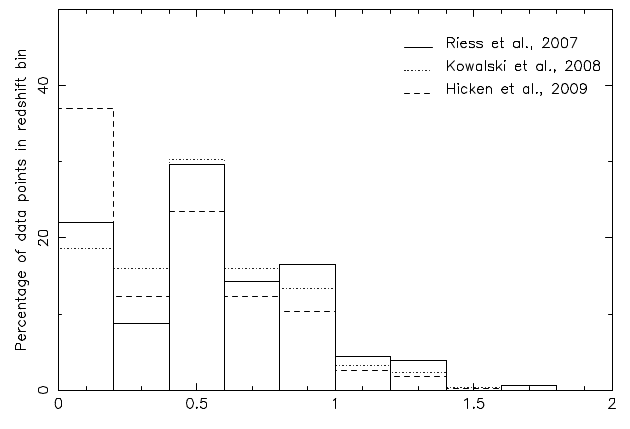
\includegraphics[]{figures/chapter3/fig3.1.png}
\caption{Percentage of SNe Ia from Gold (solid), Union (dotted) and Constitution (dashed) samples falling into redshift bins of width $\Delta z = 0.2$. There are 397 SNe Ia in the Constitution set, 307 SNe Ia in the Union compilation and 182 SNe Ia in the Gold data set. Image credit: \cite{Kwan2009} Fig. 2.}
\label{fig:3.1}
\end{figure}

Type Ia SNe are regarded as the most useful method of determining distances on cosmological scales \cite{Hicken2009}, which makes them ideal candidates for analysing distance-redshift relations. Observational data available for the study was limited: the requirements and three sets which fulfilled them are discussed in \cref{sec:3.1}. A series of projected sets were also made: \cref{sec:3.2} the same samples as the existing sets but with less error and two sets modelled on the expected capability of the \snap{}/\textsc{wfirst} mission.

\section{Observational data}
\label{sec:3.1}

Existing large-scale surveys of Ia SNe are widely used to constrain cosmological parameters, both individually (\cite{Barnes2005,Hicken2009,Kowalski2008,Riess2007}) and in conjunction with other data (\cite{LewisBridle2002,Komatsu2010}). 

The astrophysical properties required for an accurate determination of the parameters place statistical constraints on the available data and how it is processed. Leibundgut emphasises that Ia SNe are cosmologically useful precisely because they map the expansion properties of the universe over a significant fraction of its age (\cite{Leibundgut2008}), with the most recent survey \cite{Amanullah2010} providing Ia SNe luminosity distances out to $z \sim{} 1.5$ (corresponding to a look-back time of about 2/3 of the age of the universe). 
Consequently we require a catalogue of both low- and high-redshift SNe, which in practice is an amalgamation of two (or more) different surveys that require uniform calibration \cite{Kowalski2008}. Furthermore, the quality of spectroscopic data has increased rapidly since the first surveys in the mid-90s (see \cite{Leibundgut2008} for a summary) and we wish to prevent the presence of low-quality data reducing the effectiveness of the higher-quality samples. Implicit in this requirement is a divide between \lq\lq{}good\rq\rq{} and \lq\lq{}bad\rq\rq{} data, which should be made with clearly-defined criteria over all sets, rather than relying on the divides provided by the individual groups \cite{Kowalski2008}. 
Lastly, all spectroscopic data should be analysed with the same light-curve fitting model, so that magnitudes (and therefore luminosity distances) are uniformly calibrated. 

This project is concerned with the data after all of these goals is achieved: it is sufficient to state that each of the three SNe sets satisfied these properties at the time of publication. (The interested reader should consult the introduction of Kowalski’s paper \cite{Kowalski2008} for a more detailed account of how such goals are achieved in practice.) 

Three data sets (\cref{fig:3.1}) which fulfilled these requirements (selected by my supervisor) are the 2006 Gold sample of Riess et al. \cite{Riess2007}, the 2008 Union sample from the Supernova Cosmology Project \cite{Kowalski2008} and the 2009 Constitution sample from Hicken et al \cite{Hicken2009}. In early May 2010 due to \cite{Lidman2010b} I became aware of an even larger suitable set (Union 2) \cite{Amanullah2010}, but it was too late to incorporate this set directly. 

The first sample is the result of two observing periods by Riess et al. using the Advanced Camera for Surveys on the Hubble space telescope \cite{Riess2007}. The use of HST for the whole survey solves two problems: there are no atmospheric effects imprinted on the light curves \cite{Riess2007} and it there was no need to calibrate observational errors across different telescopes \cite{Leibundgut2008}. After uniform calibration and removal of local SNe ($z \lesssim{} 0.02$£, too nearby to be in the Hubble flow) the entire sample was separated into a \lq\lq{}Gold\rq\rq{} set containing SNe which had been positively identified as Type Ia using spectroscopic data and a \lq\lq{}Silver\rq\rq{} set of SNe whose type was unconfirmed \cite{Riess2007}. The Gold set comprises 182 Ia SNe of which 23 are at $z \geq{} 1$. 

The Union set of Kowalski et al. aimed to augment the existing sample of low-$z$ SNe (those in the nearby Hubble flow), since this is a region of smooth ($H(z) \sim{}$ constant) expansion, the $H(z)$ value of which was not well constrained at the time \cite{Kowalski2008}). It is mainly a uniform re-analysis of 414 SNe Ia (reduced to 307 after light-curve quality cuts) which already existed in the literature \cite{Kwan2009}: data from the first year of the two large, ground-based surveys of the time (the Supernova Legacy Survey and the ESSENCE survey) and previous surveys from a variety of instruments, including 17 SNe Ia from the Gold sample \cite{Kowalski2008}. 

The Union set is a proper subset of the Constitution set, which also contains SNe from around seven different surveys collectively known as the CfA3 set \cite{Hicken2009}. The addition of 90 Ia SNe from the CfA3 set increased the number of low-$z$ SNe by a factor of $2.6 -- 2.9$: the sample size was now sufficiently large for systematic errors to be the dominant contributor to distance modulus uncertainties \cite{Hicken2009}. According to Kwan all three data sets are consistent with one another, despite the gold set intersecting with, rather than being a subset of the other two \cite{Kwan2009}.

\section{Artificially generated data}
\label{sec:3.2}

This data falls into two categories: modification of existing data and creation of speculative projected sets. 

These represent the two major directions of future SNe cosmology: re-analysis of existing, heterogeneous data using uniform light curves and collection of new, homogeneous data from large surveys. 

The smaller-error samples (Gold 02, Union 02 and Constitution 02) were created by taking the existing data and reducing the distance modulus uncertainty $\Delta{} \mu$ fivefold. This improvement represents a reduction of systematic errors currently encountered in survey data reduction. This reduction may arise from two different areas: improvement of experimental systematics --- Malmquist bias, $k$-correction uncertainties, sample contamination with non-SNe Ia, possible gravitational lensing --- and better understanding of the SNe themselves --- different populations in different environments, evolution with redshift, possible metallicity-luminosity relation \cite{Lidman2010b}. 

Comparison of these smaller-error sets with the real ones will determine how much uncertainties in luminosity distance contribute to uncertainty in the cosmological parameters. The projected sets represent hypothetical data from the planned \textsc{wfirst} mission (previous \snap{}, then \textsc{jdem}), which has been given top priority in the recent US decadal survey \cite{Blandford2010}. The \textsc{wfirst} project consists of a space-based 1.5m telescope for photometric discovery of distant Ia SNe with ground-based spectroscopic confirmation combined with a ground-based survey of near (Hubble flow) SNe \cite{Albrecht2006}. It anticipates surveying 2000 SNe in redshifts $0.1 < z < 1.7$ \cite{Blandford2010}. The method used to generate the false data is described in \cref{sec:4.2} with the rest of the numerical work (\cref{ch:numerical-modelling}).

% chapters/modelling.tex
\chapter{Numerical Modelling}
\label{ch:numerical-modelling}

% ---------- Chapter 4: Numerical Modelling ----------

\begin{figure}[htbp]
\centering

\staticsubfigure{figures/chapter4/fig4.1a.png}{}
\hfill
\staticsubfigure{figures/chapter4/fig4.1b.png}{}

\medskip

\staticsubfigure{figures/chapter4/fig4.1c.png}{}
\hfill
\staticsubfigure{figures/chapter4/fig4.1d.png}{}

\caption{The luminosity distance-redshift relation $d_L(z)$ (top) and distance modulus curve $\mu(z)$ ($\Omega_M$, $\Omega_X$) = (1, 0), solid; (0.05, 0), dotted; and (0.2, 0.8), dashed. (bottom) for various choices of the cosmological parameters $\Omega_M$ and $\Omega_X$ : ($\Omega_M$ , $\Omega_X$ ) = (1, 0) (solid) (0.05, 0) (dotted) and (0.2, 0.8) (dashed).}
\label{fig:4.1}
\end{figure}

\begin{figure}
    \centering
    \staticsubfigure{figures/chapter4/fig4.2a.png}{}
    \hfill
    \staticsubfigure{figures/chapter4/fig4.2b.png}{}
    \caption{An example of proper maximum step size in the Markov chain.  The walk (b) completely covers the parameter space in a random order, providing a smooth posterior (a).}
\label{fig:fig4.2}
\end{figure}


\begin{figure}
\centering

\staticsubfigure{figures/chapter4/fig4.3a.png}{}
\hfill
\staticsubfigure{figures/chapter4/fig4.3b.png}{}

\medskip

\staticsubfigure{figures/chapter4/fig4.3c.png}{}
\hfill
\staticsubfigure{figures/chapter4/fig4.3d.png}{}

\caption{Examples of improper maximum step sizes in the Markov chain. An incorrect step size causes the chain to inefficiently cover the parameter space: too small and the chain remains stuck in a small area, too large and the chain oscillates between maxima. The walks (d), (b) clearly show the problem, whereas the effect on the distributions (c), (a) is more subtle.}
\label{fig:4.3}
\end{figure}

The computational work involves four stages: writing appropriate code; the creation of SNe data; implementation of the Markov Chain Monte Carlo (\mcmc{}) method; creation of credible regions from the prior probabilities generated by \mcmc{}. The codes to do so are shown in \cref{tab:programs-written}. The programming language which I chose was \matlab{} due to its efficient handling of large arrays and the (relative) simplicity of generating visualisations of the data.\footnote{For a larger number of parameters or longer walks the low-level language Fortran is a more suitable program.}

\begin{table}[htbp]
\centering

\begin{threeparttable}
\caption{Programs written for the project.}
\label{tab:programs-written}

\begin{tabular}{@{} l l p{8cm} @{}}
\toprule
Filename & Type & Purpose \\
\midrule

\texttt{conf1} & Program &
Comparison of credible regions of single-parameter models for all data sets from Markov chains. \\

\texttt{conf2} & Program &
Visualisation of credible regions of 2 or 3 parameters for one data set from Markov chains. \\

\texttt{credibleregions} & Subfunction of \texttt{conf2} &
Calculation of credible regions for one parameter from Markov chains. \\

\texttt{friedmann} & Function &
Calculation of $\mu(z)$ from numerical integration of the Friedmann equations given a 5-tuple of parameters and an array of redshifts. \\

\texttt{friedmann\_rhs} & Subfunction of \texttt{friedmann} &
Array storing the ODEs to be solved. \\

\texttt{likelihood} & Function &
Global likelihood calculation from the $\mu(z)$ array generated by \texttt{friedmann}. \\

\texttt{montecarlo} & Program &
Implementation of the Metropolis--Hastings algorithm and generation of histograms and random walk plots. \\

\bottomrule
\end{tabular}

% Uncomment when table notes are needed.
% \begin{tablenotes}
% \footnotesize
% \item[a] Example table note.
% \end{tablenotes}
\end{threeparttable}
\end{table}


\section{Codes written for the project}
\label{sec:codes-written}

The codes required for the project varied widely in complexity (and consequently in debugging time). I wrote the codes starting with the clearest structure, then optimising them for speed. Two modifications caused the greatest increase in efficiency: firstly the replacement of for-loops with array operations; secondly minimising the memory used when writing data to files. Despite these measures, generating the Markov chains remained demanding in terms of computer time and hardware (\cref{sec:4.1.3}).

\subsection{Numerical solution of the Friedmann equations}
\label{sec:4.1.1}

The function designed to calculate $\mu(z)$ by solving the scaled Friedmann equations \cref{eq:2.7} was \texttt{friedmann}. The function calculated the initial conditions for the ODEs and passed them to the inbuilt \matlab{} ODE solver \texttt{ode45} along with the right hand side of the equations which were contained in the subfunction \texttt{friedmann\_rhs}. The output from the ODE solver was a 4 column array $\left[ \Omega_m (z_i), \Omega_X (z_i), H(z_i), D_L(z_i)\right]$, from which $D_L(z_i)$ was extracted to find $\mu(z_i)$ according to \cref{eq:1.13}.

The output of \texttt{friedmann} was the 2-column array of distance modulus versus redshift $[z_i \,, \mu(z_i)]$. Plotting this generated a redshift-distance modulus curve. I compared my own results \cref{fig:fig4.1b} and \cref{fig:fig4.1d} to those \cref{fig:fig4.1a} and \cref{fig:fig4.1c} published by Hogg in \cite{Hogg2000} to ensure that \texttt{friedmann} produced correct $d_L(z)$ and $\mu(z)$ values. Due to the assumption of a flat spatial geometry (with $\Omega_m + \Omega_X = 1$) I could not produce the curve for $(\Omega_m = 0.05, \, \Omega_X = 0)$. Therefore I was able to verify that the script both correctly solved the Friedmann equations and correctly converted from the distance-redshift relation to the observed quantity given in the data.

\subsection{Likelihood calculations}
\label{sec:4.1.2}

The random walk requires the calculation of the likelihood $L(x)$ at each selected point $x$ in the parameter space. The point with the largest likelihood corresponds to the set of parameter values which are most likely to have generated the $\mu(z)$ curve formed from the data.   The analytical value \cref{eq:4.1} for $L(x)$ is the product of the likelihood according to each point $\mu(z_j)$ in the data. Since the error in $\mu$ is well-characterised by a Gaussian distribution, the individual likelihoods are \cref{eq:4.1} where at the redshift $z_j$ , $\sigma$ is the standard deviation of the uncertainty in the distance modulus measurement $\mu(z_j)$ (this was provided explicitly in the data) and $\mu(x)$ is the distance modulus calculated by the model with parameter 5-tuple $x$. The individual likelihood is maximised for the curve which, at each $z_j$ in the chosen SNe data set, matches as closely to the distance modulus $\mu_j$ of the SN there, i.e. when $\mu(x) - \mu(z_j) = 0$.

% Equation (4.1)
\begin{equation}
    \mathcal{L}(x)
    = \prod_{j} \mathcal{L}_{j}(x)
    \quad
    \text{where}
    \quad
    \mathcal{L}_{j}(x)
    = \mathcal{L} \left( \mu{} ( z_{j};x ) \right)
    = \frac{1}{\sqrt{2\pi{}\sigma{}}} \exp 
    \left( 
        - \frac{\left( \mu{} (x) - \mu{} (z_{j}) \right)^{2]}}{2 \sigma{}^{2} }
    \right)
\label{eq:4.1}
\end{equation}

Since the global likelihood is the product of Gaussians, computational accuracy is maximised by calculating the logarithms of the individual values to avoid overflow. To perform global likelihood calculations for each set of parameter values I wrote a subfunction called likelihood rather than using a pre-written \matlab{} routine. The scalar output from likelihood was passed to the main program which used this and the previous value to determine the next model to pick in parameter space as described in \cref{alg:2.1}.

\subsection{The Metropolis-Hastings algorithm}
\label{sec:4.1.3}

The Metropolis-Hastings algorithm (\cref{alg:2.1}) is a random walk which produces Markov chains that accept or reject a proposed step on the basis of the likelihood ratio between the steps. The main program \texttt{montecarlo} looped over each maximum step size, performing the Metropolis-Hastings algorithm for a given walk length, writing the parameter values and likelihood to file at each step, before creating a histogram and a line graph for each of the varying parameters in the walk. The algorithm contains three computationally important factors: the number of steps in the walk, the dimensionality of the parameter space and the size of the neighbourhood around each point. As discussed in \cref{sec:4.3}, although writing the code is straightforward, ensuring that it truly approximates the posteriors from the longer crude Monte Carlo method is not so simple.


\section{Generation of the projected WFIRST set}
\label{sec:4.2}

The projected \textsc{wfirst} data is designed to illustrate improvements in constraints on the parameters given a larger Ia SNe data set from a single survey. The first step in making the projected data was to generate 2000 redshifts from a random distribution $0.1 < z < 1.7$ using \texttt{randn}, a built-in \matlab{} (pseudo-)random number generator. The Friedmann integrator (\cref{sec:4.1.1} calculated the distance moduli at each redshift. 

Two types of errors were now introduced: those due to the instrument and those from uncontrollable sources. The first arises from the photometric calibration and is estimated by the Dark Energy Task Force report in \cite{Albrecht2006} to be a linear function of redshift $k(1 + z)$, with $k$ a constant between $0.01$ for an \lq\lq{}optimistic\rq\rq{} view and $0.05$ for a \lq\lq{}pessimistic\rq\rq{} one. Since other errors are not quantified by the working group, I estimated them from the most recent SNe survey, the Union 2 compilation \cite{Amanullah2010}. These additional errors (potentially arising from a variety of sources discussed in \cref{sec:3.1} and \cite{Leibundgut2009,Lidman2010b}) were assigned by random selection from the Union2 set to the artificial SNe. The total uncertainty in the distance moduli is then the sum of the systematic error and the random error estimates. Each data point was then displaced from the concordance model curve by the error bar size multiplied by a random number from $[-1, 1]$. Two sets were made: the snap (snap 02) set using the pessimistic (optimistic) error from the JDEM report and the same magnitude ($0.2x$ magnitude) errors as the Union2 survey, maintaining the scaling of the quantified errors.

\section{Simulation of the posterior distributions}
\label{sec:4.3}

The posterior distributions for each Ia SNe compilation and model are approximated by histograms created using the Metropolis-Hastings version of Markov chain Monte Carlo. The requirements for a reasonable approximation to the true (unknown) posterior are:

\begin{itemize}
    \item Sufficient burn-in time for the chain to reach an equilibrium.
    \item A suitable maximum step size to explore the parameter space.
    \item Initial conditions (a \lq\lq{}zero-parameter model\rq\rq{}) which do not introduce bias into the walks.
\end{itemize}

Ensuring that all these conditions were met without resorting to highly complex code and parallel computing was a non-trivial task involving much trial and error. This constituted the majority of the project: although simulations were started in May, only 4065 hours of CPU time actually produced data suitable for further processing.\footnote{The output files were timestamped so that it was possible to tell the duration of the walk.} The rest of the time was spent discovering the aforementioned problems in practice, rewriting the code and running new simulations to determine whether the issue had been resolved. 

In this section, I examine the problems faced in more detail and outline the methods used to ameliorate them. The convergence length of the Markov chain cannot be predetermined. Although the \mcmc{} formalism guarantees convergence for most PDFs, it places no bounds on the number of iterations required before convergence is achieved \cite{Gregory2005,Dunkley2005,Christensen2001}. Existing methods are empirical: one runs a series of tests for non-convergence, the negative results of which imply---but do not confirm---that the chain has converged \cite{Christensen2001}. These methods, which include using second-order Markov chains to calculate a bound on the accuracy of the estimations and comparing the values from multiple chains \cite{Dunkley2005}, were considered unnecessary for such a small number of parameters (compared to eleven or more in \cmb{} calculations \cite{LewisBridle2002}). Instead, following \cite{Gregory2005}, the burn-in time preceding convergence was estimated at $1\%$ of the total walk length, provided that the posterior produced was smooth. 

After some experimenting to find a smooth histogram of $\Omega_m$ from the Constitution compilation, the initial walk length estimate of $5 \times 10^4$ steps was increased to $1 \times 10^5$ for the smaller-error observational data (Constitution 0.2, Gold 0.2, Union 0.2) and $2 \times 10^5$ for the projected sets (Snap, Snap 0.2) for one-parameter models. The number of steps required to produce smooth posteriors scales with the dimensionality of the parameter space: (approximately) linearly for \mcmc{} methods \cite{Dunkley2005} compared to exponentially in the crude MC scenario \cite{Christensen2001}. In practice, this linear scaling is not achieved \cite{Christensen2001,Dunkley2005,LewisBridle2002}. Therefore a balance between smoothness and running time was estimated by multiplying the one-parameter walk length tenfold for each additionally varying parameter. The exception to this was multiple-parameter models involving the time-varying dark energy equation of state $w_1$, which had a long burn-in time: these walks had to be redone with twice the existing steps for smoothness. Computational efficiency required that the total number of steps in the chain was both sufficiently large to widely explore the parameter space (\cref{fig:fig4.2b}) and sufficiently small that the program runs in a sensible amount of time given the time span available for the project. 

The second problem in the algorithm is the possibility of sampling bias introduced by the the neighbourhood size. This is governed by a maximum step size: the actual steps will be a fraction of this (depending on the random multiplier chosen). If the maximum step is too small, the walk does not leave a small subset of the parameter volume (\cref{fig:fig4.3b}). Consequently, it will show fine detail (\cref{fig:fig4.3a}), but only in a small section of the characteristic width, leading to an incorrect posterior. Conversely, if the step size is too large, the chain (\cref{fig:fig4.3d}) will oscillate between regions of high likelihood (\cref{fig:fig4.3c}) without exploring the parameter space in-between. This results in a posterior which sparsely outlines peaks in the likelihood, but does not give any accurate shape to the rest of the space. Thus the same initial conditions can produce two very different chains if different maximum step sizes are selected. Although a method called parallel tempering \cref{sec:6.1} exists which efficiently covers the parameter space using information from a variety of step sizes, it was too complex to implement in this project. Consequently the walk had to be repeated for each model over a range of different step sizes incremented by factors of two using a for-loop. It became evident that there was no step size which was suitable for all parameters, e.g. the Hubble parameter $h$ required a small step because of the small characteristic width of its prior, whereas the dark energy equation of state parameters $w_0$ (constant) and $w_1$ (time-varying) produced smooth walks with much larger step sizes. The core step sizes were $0.1 \times 2k ,\, k \in {-2, -1, 0, 1, 2}$ and additional sizes were added after the walks from these were examined: if the $0.025$ step was too large then one of $0.0125$ was run; if the $0.4$ step was too small, steps of $0.8$ and even $1.6$ were run.

The final issue to address is the choice of initial conditions for the walk. If the initial conditions were too far from the likely parameter values then a large number of steps would be wasted as burn-in time: the section of the walk in which the chain travels towards high-likelihood regions \cite{Gregory2005}. Consequently the initial conditions chosen corresponded to the concordance ($\Lambda$CDM) model, an accepted estimate to the correct values of the cosmological parameters \cite{Hartle2003}. The values of the concordance model vary slightly from reference to reference: I adopted the 1-significant figure values used in \cite{Hartle2003}: $\Omega_m = 0.3; w_0 = \Lambda = -1$; with the addition of $w_1 = \gamma = 0$ (by definition the concordance model has neither time-variation in the dark energy equation of state nor interaction). I chose to write the Hubble constant parameter as $h/h_{72}$ so that a value of 1 gave $H_0 = 72\,\mathrm{km}\,\mathrm{s}^{-1}\,\mathrm{Mpc}^{-1}$ , the current best estimate for $H_0$ \cite{Riess2009}.

Once all three criteria were met, the Markov chains produced use approximations to the true posterior PDFs. This enabled the smooth walks with suitable step sizes (\cref{fig:fig4.2}) to be selected for the next stage in the project: finding credible regions.


\section{Credible regions from posteriors}
\label{sec:4.4}

Not all of the histograms from the Markov chains were reasonable approximations to the posterior PDFs for that model. I categorised all successful Markov chain histograms:
\begin{equation*}
    (\text{8 data sets})
    \times
    \left[
        \binom{4}{2} 
        +
        \binom{4}{1}
    \right] \text{models}\footnote{The zero-parameter model is $\Lambda$CDM.}
    \times
    (\text{6 step sizes})
    =
    8 \times (6+4) \times 6
    =
    480\ \text{histograms}.
\end{equation*}
as unsuitable (maximum step size either too small or too large) or suitable (satisfying all three criteria). I then selected the smoothest histograms (if there were multiple maximum step sizes which produced a good result) for further analysis. The next step in the analysis was the creation of credible regions for 1d and 2d subspaces of the 5d parameter space.

\subsection{Credible regions for individual parameters}
\label{sec:4.4.1}

Although we desire a single estimate for each parameter, the posteriors are not delta functions, so there is an inherent width to the high-probability region whence the \lq\lq{}best fit\rq\rq{} estimate is selected. To examine the posterior PDFs in greater detail, I wrote the graphing program conf1. This read in the Markov chain data from a set of files and output line graphs of each posterior. The process involved binning the data, ordering the bins by population, then selecting those regions within which lay $68\%$, $95\%$ and $99\%$ of the points in the chain. These regions were plotted as line graphs shaded according to increasing probability content. The mode and standard deviation were also plotted as a point with errorbars above the curve. Thus I was able to facilitate comparison between the different data sets.

\subsection{Credible regions for multiple parameters}
\label{sec:4.4.2}

Models with more than one free parameter can be examined in a similar manner to those with only a single free parameter. Although the theory is the same, the binning is based upon the values of all parameters simultaneously. Therefore I needed to write not only a program to generate contour maps of the credible regions (\texttt{conf2}) but also one to calculate them (\texttt{credibleregions}). Since the Metropolis- Hastings algorithm moves in all directions within the 2d parameter space, the value of both parameters is related. Unlike the existing \matlab{} function \texttt{histc}, which bins the parameter values in the random walk independently of one another, \texttt{credibleregions} bins the 2d subspace according to each pair of values. This retained any patterns in the walk, allowing me to look for correlations between parameters.

% chapters/results.tex
\chapter{Results}
\label{ch:results}

% ---------- Chapter 5: Results ----------

\begin{table}
\centering

\begin{threeparttable}

\caption{
Best-fit parameters for single-parameter models to SNe Ia data.
The accuracy of the results is limited to $1\times10^{-3}$ due to
the grid spacing.
}
\label{tab:5.1}

\small

\begin{tabular}{@{}lccccc@{}}
\toprule

SNe Ia sample
&
$\Omega_M$
&
$w_0$
&
$w_1$
&
$\gamma$
&
$H_0$\tnote{c}
\\

\midrule

Constitution\tnote{a}
&
$0.29 \pm 0.02$
&
$-1.0 \pm 0.06$
&
$-0.26 \pm 0.4$
&
$0.06 \pm 0.1$
&
$64.95 \pm 0.2$
\\

Constitution 0.2x\tnote{a}
&
$0.29 \pm 0.01$
&
$-1.0 \pm 0.01$
&
$-0.24 \pm 0.07$
&
$0.07 \pm 0.03$
&
$65.01 \pm 0.03$
\\

Gold\tnote{a}
&
$0.34 \pm 0.04$
&
$-0.92 \pm 0.1$
&
$0.73 \pm 0.7$
&
$-0.33 \pm 0.3$
&
$63.55 \pm 0.3$
\\

Gold 0.2x\tnote{a}
&
$0.34 \pm 0.01$
&
$-0.92 \pm 0.02$
&
$0.73 \pm 0.1$
&
$-0.32 \pm 0.05$
&
$63.6 \pm 0.06$
\\

Union\tnote{a}
&
$0.29 \pm 0.03$
&
$-1.1 \pm 0.08$
&
$-0.24 \pm 0.5$
&
$0.04 \pm 0.2$
&
$69.68 \pm 0.3$
\\

Union 0.2x\tnote{a}
&
$0.29 \pm 0.01$
&
$-1.1 \pm 0.02$
&
$-0.24 \pm 0.08$
&
$0.03 \pm 0.03$
&
$69.76 \pm 0.04$
\\

SNAP\tnote{b}
&
$0.30 \pm 0.01$
&
$-1.0 \pm 0.02$
&
$0.01 \pm 0.1$
&
$0.0 \pm 0.04$
&
$72.05 \pm 0.1$
\\

SNAP 0.2x\tnote{b}
&
$0.30 \pm 0.01$
&
$-1.0 \pm 0.01$
&
$0.0 \pm 0.02$
&
$0.0 \pm 0.01$
&
$72.01 \pm 0.03$
\\

\bottomrule
\end{tabular}

\begin{tablenotes}
\footnotesize

\item[a]
Results obtained using the published supernova compilations.
The value of $H_0$ used in the original calibration is not known.

\item[b]
Results obtained using data sets generated with
$H_0 = 72\ \mathrm{km\,\mathrm{s}^{-1}\,\mathrm{Mpc}^{-1}}$.

\item[c]
Converted from the fitted quantity $h/h_{72}$ using
$H_0 = 100 \left( h/h_{72} \right) \times 72 \mathrm{km}\,\mathrm{s}^{-1}\,\mathrm{Mpc}^{-1}$.
The values of $h/h_{72}$ were recorded to an accuracy of $ 1 \times 10^{-3}$.

\end{tablenotes}

\end{threeparttable}

\end{table}


\begin{table}[htbp]
\centering

\begin{threeparttable}

\caption{
Comparison of best-fit values and 68\% confidence levels with values
quoted in the original SNe surveys. The accuracy of the results is
limited to $1\times10^{-3}$ due to the grid spacing.
}
\label{tab:5.2}

\begin{tabular}{@{}lccc@{}}

\toprule

\multirow{2}{*}{Compilation}
&
\multicolumn{3}{c}{Parameter value $\Omega_M$}
\\

\cmidrule(lr){2-4}

&
Survey
&
Own results
&
Reduced-error set
\\

\midrule

Constitution &
$0.281^{+0.037}_{-0.016}$ &
$0.291 \pm 0.02$ &
$0.290 \pm 0.01$
\\

Gold\tnote{a} &
$0.28 \pm 0.04$ &
$0.342 \pm 0.04$ &
$0.342 \pm 0.01$
\\

Union &
$0.287^{+0.029}_{-0.027}\,\text{(stat)}
^{+0.039}_{-0.036}\,\text{(sys)}$ &
$0.285 \pm 0.03$ &
$0.287 \pm 0.01$
\\

\midrule

\multirow{2}{*}{Compilation}
&
\multicolumn{3}{c}{Parameter value $w_0$}
\\

\cmidrule(lr){2-4}

&
Survey
&
Own results
&
Reduced-error set
\\

\midrule

Constitution &
$-0.913^{+0.066}_{-0.068}\,\text{(stat)}
\pm 0.11\,\text{(sys)}$ &
$-1.03 \pm 0.06$ &
$-1.03 \pm 0.01$
\\

Gold &
$-0.8^{+0.6}_{-1.0}$ &
$-0.934 \pm 0.1$ &
$-0.928 \pm 0.02$
\\

Union &
$-0.969^{+0.059}_{-0.063}\,\text{(stat)}
^{+0.063}_{-0.066}\,\text{(sys)}$ &
$-1.07 \pm 0.08$ &
$-1.06 \pm 0.02$
\\

\bottomrule

\end{tabular}

\begin{tablenotes}
\footnotesize
\item[a] Gold set assumes a priori $\Omega_M = 0.28 \pm 0.04$.
\end{tablenotes}

\end{threeparttable}

\end{table}


\begin{table}[htbp]
\centering

\begin{threeparttable}

\caption{One-parameter deviations from the $\Lambda$CDM values from the results in
\cref{sec:5.1}. ``Gold'' is the best-fit values from the Gold sample;
``Const./Union'' is the average of the best-fit values from the two data sets;
``Compromise'' is the average of all three and ``WMAP+BAO+Const.'' represent the
most up-to-date estimates from CMB, BAO and the Constitution set, copied from
\cite{Komatsu2010}. Uncertainties quoted are 68\% CL for Gold and WMAP+BAO+Const.
and the standard error of the 68\% CL for the other two columns.}
\label{tab:5.3}

\begin{tabular}{@{}lcccc@{}}
\toprule
Parameter & Gold\tnote{a} & Const./Union & Compromise & WMAP+BAO+Const. \\
\midrule

$\Omega_M$ &
$0.34 \pm 0.04$ &
$0.29 \pm 0.03$ &
$0.31 \pm 0.02$ &
$0.282^{+0.015}_{-0.016}$ \\

$w_0$ &
$-0.92 \pm 0.1$ &
$-1.1 \pm 0.07$ &
$-1.0 \pm 0.06$ &
$-0.980 \pm 0.053$ \\

$w_1$ &
$0.73 \pm 0.7$ &
$-0.25 \pm 0.45$ &
$0.08 \pm 0.39$ &
$0.38^{+0.66}_{-0.65}$ \\

$\gamma$ &
$-0.33 \pm 0.3$ &
$0.05 \pm 0.16$ &
$-0.08 \pm 0.15$ &
$0$ by definition \\

\bottomrule
\end{tabular}

\begin{tablenotes}
\footnotesize
\item[a] Sign of $w_0$ corrected from a misprint in the original source.
\end{tablenotes}

\end{threeparttable}

\end{table}


The project produces four different outputs for each data set: the Markov chains used to produce the posterior PDFs, the posteriors themselves, credible regions for the $\binom{4}{1}$ parameters and $\binom{4}{2}$ pairs thereof and the distance modulus curves for those parameter values which have the greatest likelihood. Of these, the latter two are useful for analysis. It is also desirable to compare the results from this project to those obtained by the supernova search teams themselves and by alternative methods of parameter estimation, namely anisotropies in the cosmic microwave background and baryon acoustic oscillations in elliptical galaxies. For one of the models to be a viable alternative we require that the best-fit values from all of the observational data sets agree, i.e. they all lie within the others’ 68\% credible regions. This is due to the lack of tension between the three Ia SNe sets asserted by \cite{Kwan2009}: if the data from all observations are consistent, then those parameters which have a high probability of producing one set’s distance moduli must also have a high probability of producing the others. Conversely, if the credible regions from the three observational sets do not overlap in a certain subspace, then we may discard the subset of models which span that subspace. This is a qualitative measure which may be quantitatively expressed by calculating the Bayes factors from the posteriors, using a technique described in the further work (\cref{sec:6.1}). 

Firstly we examine the credible regions from the single-parameter models in \cref{sec:5.1}. (For brevity I omit similar analysis for the individual parameters in two-parameter models.) I then examine the possibility of correla- tions between parameters shown in the two-parameter models in \cref{sec:5.2}. In \cref{sec:5.3} I add \bao{} results from the Sloan Digital Sky Survey and \cmb{} results from the seven-year Wilkinson Microwave Anisotropy Probe to the 2d credible regions in order to obtain tighter constraints on the cosmological parameters. Lastly in \cref{sec:5.4} I examine the astrophysical and cosmological implications of a non-$\Lambda$CDM universe.

\section{Parameter values from 1-dimensional models}
\label{sec:5.1}

\begin{figure}
\centering
\staticfigure[.8\textwidth]{figures/chapter5/fig5.1a-f.png}{Posterior PDFs for each parameter in the single-parameter models (not marginalised over $H_0$). Each data set is denoted by a different colour, with the $1\sigma$ credible region in the lightest shade and $3\sigma$ the darkest. Regions in black are outside $3\sigma$. Larger versions of the $1\sigma$ credible regions are contained in \cref{app:large-figures}. (b) shows the Hubble parameter $h/h_{72}$, (c) the matter density $\Omega_m$ ; (d) the constant equation of state parameter $w_0$; (e) the varying equation of state parameter $w_1$; and, (f) the mixing factor $\gamma$.}
\end{figure}

The single-parameter models represent the simplest modification to the concordance $\Lambda$CDM model, containing only matter (both baryonic and dark) and a cosmological constant. Each posterior represents the probability that a value from the continuum set by the prior is the value which created the data. Thus, the mode is the value with the highest likelihood of being the value in the observable universe. The error is taken to be the width of the 68\% credible region by convention. The results are summarised in \cref{tab:5.1}. Plotting the credible regions themselves (\cref{fig:fig5.1a-f}) allows a comparison of the 1$\sigma$, 2$\sigma$, 3$\sigma$ errors for each data set.
   
The first step is to determine the value of $H_0$ used by the different SNe observing groups. This serves two purposes: it acts as a plausibility check on the smaller-error data (since these sets should agree (i.e. their 1$\sigma$ intervals should overlap) with the $H_0$ value of the sets on which they are based) and it justifies the use of the Hubble parameter as a free parameter for all models. If the $H_0$ value were the same for all data sets, I would have been able to set it as a constant, thus reducing the dimensionality of the model parameter spaces and shortening the length of the Markov chains. We find in \cref{fig:fig5.1a-f}(b) and \cref{tab:5.1} that only between the Gold and Constitution sets is there overlap in the 3$\sigma$ regions and that the credible regions of each reduced-error set are entirely enclosed by the same regions in the corresponding original set. Therefore we can conclude that a different value for the Hubble constant was applied to each normal-error set and that the reduced-error sets are behaving plausibly. It is vital to stress that I have not discovered a value for the Hubble constant: these values were applied arbitrarily by the different SNe search teams and then marginalised over as a nuisance parameter. This is in contrast to the other credible regions, which do suggest a value for their parameters.

The single-parameter models indicate that only minor modifications to the concordance model produce a better fit to the observed data. All three posteriors from the observational data give parameter values with consistent agreement, i.e. the 1$\sigma$ confidence regions overlap. 

The cosmological matter density $\Omega_m$ (\cref{fig:fig5.1a-f}(c)) has a best-fit value of $0.29$ across the Constitution and Union sets and their reduced-error sets and this agreement is confirmed by the overlap of the $1\sigma$ regions. The Gold set $1\sigma$ region intersects the $1\sigma$ regions of the Constitution and Union sets at $\Omega_m = 0.31$, however one must look at the 2$\sigma$ confidence regions before an agreed value is found between these and the Gold 0.2x set. The Gold and Gold 0.2x sets have a best-fit parameter value of $\Omega_m$ = 0.34, which is ruled out at 3$\sigma$ for the Constitution and Union sets and 4$\sigma$ for the corresponding 0.2x error sets. This demonstrates that the smaller-error sets amplify the calibration differences between the Gold set and the later Constitution and Union sets.

Similarly, the constant parameter $w_0$ (\cref{fig:fig5.1a-f}(c)) in the dark energy equation of state is well-agreed upon by all three observational data sets, which display overlap in their $1\sigma$ credible regions at $w_0 = -1$, although one must go to $2\sigma$ for overlap between the $1\sigma$ Gold 0.2x region and either the Constitution or Union sets. Once again the Gold 0.2x set does not overlap with the other two reduced-error sets. The agreement between the Constitution and Union samples is not as clear as for the matter density, as their best-fit values no longer agree, nor is there overlap at $1\sigma$ between their reduced-error sets. Nevertheless, the considerable overlap between the normal-error sets suggests that a cosmological constant $w_0 = -1$ can produce the observed SNe data.
   
There is no clear value for a time-varying dark energy equation of state which would better explain the distance moduli from the SNe data. This is once again due to the lack of consistency between the Gold set and the Union and Constitution sets. The latter two sets and their reduced-error sets all have a best-fit value around $w_1 = -0.25$ \cref{tab:5.1} whereas the Gold and Gold 0.2x sets share a best-fit value of $w_1 = 0.73$. The Gold best-fit value is ruled out at $3\sigma$ by the other two sets, whose best-fit value is slightly more plausible, lying in the 2$\sigma$ region for the Gold set. The 1$\sigma$ regions for all three observed sets intersect at $w_1 = 0.2$ in \cref{fig:fig5.1a-f}(e) whereas the concordance value of $w_1 = 0$ is in the 2$\sigma$ region for the Gold set. This suggests the inclusion of a small, positive variation in the equation of state. Given the difference in best-fit values between the Gold set and either the Constitution and Union sets, any modification would need to be tested against a sample of SNe at higher redshift (when the time-varying parameter has greater effect) to ascertain which of $w_1 \sim -0.25$, $w_1 \sim 0.2$ or $w_1 \sim 0.73$ is the most suitable value.
   
The interaction parameter $\gamma$ in \cref{fig:fig5.1a-f}(f) presents the same dilemma: although there is overlap of the 1$\sigma$ credible regions for the Gold and Union sets (the Constitution and Gold sets intersect at their 1 - 2$\sigma$ boundaries), the best-fit values lie in the 2$\sigma$ region of the other set. The considerable overlap between the Constitution and Union sets and their respective reduced-error sets is again present, all of which prefer (Table 5.1) a small positive interaction parameter to none at all. In contrast the Gold and Gold 0.2x sets prefer a negative interaction parameter approximately one order of magnitude greater than the Union and Constitution sets’ best-fit value. Thus the observational data propose a contradicting energy transfer: $\gamma > 0$ represent the transfer of energy from dark energy into matter, whereas $\gamma < 0$ represents the opposite. There is no clear value which satisfies all observational sets.

The projected sets from the \snap{} survey were artificially generated, so they do not propose parameter values for the observable Universe. As with the $H_0$ credible regions, we are interested solely in the reproduction of the values used to generate the distance moduli and the width of the region compared to the other data sets. From \cref{tab:5.1} we see that both the normal and reduced-error sets display the same best-fit values: moreover, these correspond to the concordance model values which were used to generate the data. This demonstrates that the Markov chains were run for a sufficient time to achieve convergence with the true posterior (i.e. stable equilibrium). Although the Snap 0.2x set display 1$\sigma$ regions which are far narrower than the other data sets, the Snap errors are of the same order of magnitude as those of the reduced-error sets. This suggests that a recalibration of existing data which reduces fivefold the uncertainty in distance moduli may produce equally tight constraints on the cosmological parameters as the pessimistic view of results from a new survey.

Comparison to the original papers in \cref{tab:5.2} is reassuring: the posteriors do not contradict the existing results for the Union and Constitution sets. Unfortunately, the tension in single-parameter models between the Gold set and these two sets is not reproduced in the original papers. This is because their value for the matter density was fixed at $\Omega_m = 0.28 \pm 0.04$, rather than the 0.3 which I used, so their constraints on the dark energy equation of state cannot be readily compared (\cite{Riess2007}). Their decision to use $\Omega_m$ as a Gaussian prior with maximum at 0.28 and width 0.04 came from large-scale structure measurements to obtain $\Omega_m$ h and Cepheids (another type of standard candle) to find a value for $H_0$ \cite{Riess2007}, so the validity of their results are sensitive to changes in the accepted values for $H_0$ . Therefore it is difficult to obtain a meaningful comparison between my single-parameter results and those of Riess et al. The 0.2x sets produce narrower confidence intervals due to the scaling of the error bars and the same best-fit values because they share the same data points as the observed data. Although this situation is less than ideal because the errors which contribute to the $\mu(z)$ uncertainties also produce scatter in the data points, there was no information available to guide any ”correction” to this scatter, so alterations would have generated meaningless data. The reproduction of best-fit values acts as a ”sanity check” to confirm convergence of the Markov chains. Quantitative attempts to compare how the parameter uncertainties scale with those in the distance moduli are limited by the resolution of the binning. Nevertheless, for both the normal- and reduced-error sets, my best-fit results do fit within and the 1$\sigma$ limits do overlap with (where comparison is appropriate) the 1$\sigma$ limits quoted in the papers.


\section{Degeneracies between parameters from 2-dimensional models}
\label{sec:5.2}

\begin{figure}
\centering

\staticsubfigure{figures/chapter5/fig5.2a.png}{Constitution}
\hfill
\staticsubfigure{figures/chapter5/fig5.2b.png}{Union}

\medskip

\staticsubfigure{figures/chapter5/fig5.2c.png}{Gold}
\hfill
\staticsubfigure{figures/chapter5/fig5.2d.png}{SNAP}

\caption{Credible regions illustrating correlations between the matter density and constant equation of state parameter for the different data sets: (a) Constitution; (b) Union; (c) Gold; and (d) SNAP.}
\label{fig:fig5.2}
\end{figure}

\begin{figure}
\centering

\staticsubfigure{figures/chapter5/fig5.3a.png}{Constitution}
\hfill
\staticsubfigure{figures/chapter5/fig5.3b.png}{Union}

\medskip

\staticsubfigure{figures/chapter5/fig5.3c.png}{Gold}
\hfill
\staticsubfigure{figures/chapter5/fig5.3d.png}{SNAP}

\caption{Credible regions illustrating correlations between the matter density and varying equation of state parameter for the different data sets: (a) Constitution; (b) Union; (c) Gold; and (d) SNAP.}
\label{fig:fig5.3}
\end{figure}

\begin{figure}
\centering

\staticsubfigure{figures/chapter5/fig5.4a.png}{Constitution}
\hfill
\staticsubfigure{figures/chapter5/fig5.4b.png}{Union}

\medskip

\staticsubfigure{figures/chapter5/fig5.4c.png}{Gold}
\hfill
\staticsubfigure{figures/chapter5/fig5.4d.png}{SNAP}

\caption{Credible regions illustrating correlations between the matter density and interaction parameter for the different data sets: (a) Constitution; (b) Union; (c) Gold; and (d) SNAP.}
\label{fig:fig5.4}
\end{figure}

\begin{figure}
\centering

\staticsubfigure{figures/chapter5/fig5.5a.png}{Constitution}
\hfill
\staticsubfigure{figures/chapter5/fig5.5b.png}{Union}

\medskip

\staticsubfigure{figures/chapter5/fig5.5c.png}{Gold}
\hfill
\staticsubfigure{figures/chapter5/fig5.5d.png}{SNAP}

\caption{Credible regions illustrating correlations between the constant and varying equation of state parameters for the different data sets: (a) Constitution; (b) Union; (c) Gold; and (d) SNAP. The black line marks the ``CMB wall'' $w_0 + w_1 = 0$.}
\label{fig:fig5.5}
\end{figure}

\begin{figure}
\centering

\staticsubfigure{figures/chapter5/fig5.6a.png}{Constitution}
\hfill
\staticsubfigure{figures/chapter5/fig5.6b.png}{Union}

\medskip

\staticsubfigure{figures/chapter5/fig5.6c.png}{Gold}
\hfill
\staticsubfigure{figures/chapter5/fig5.6d.png}{SNAP}

\caption{Credible regions illustrating correlations between the constant equation of state and interaction parameters for the different data sets: (a) Constitution; (b) Union; (c) Gold; and (d) SNAP.}
\label{fig:fig5.6}
\end{figure}

\begin{figure}
\centering

\staticsubfigure{figures/chapter5/fig5.7a.png}{Constitution}
\hfill
\staticsubfigure{figures/chapter5/fig5.7b.png}{Union}

\medskip

\staticsubfigure{figures/chapter5/fig5.7c.png}{Gold}
\hfill
\staticsubfigure{figures/chapter5/fig5.7d.png}{SNAP}

\caption{Credible regions illustrating correlations between the varying equation of state and interaction parameters for the different data sets: (a) Constitution; (b) Union; (c) Gold; and (d) SNAP.}
\label{fig:fig5.7}
\end{figure}

\begin{figure}
\centering
\begin{minipage}[c]{0.48\textwidth}
  \centering
  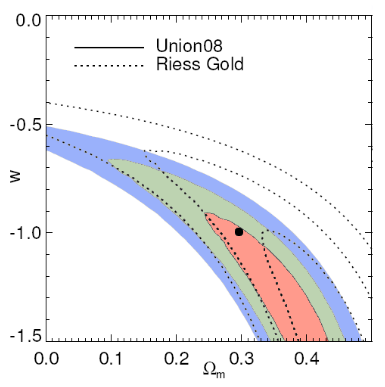
\includegraphics[width=\linewidth]{figures/chapter5/fig5.8.png}
\end{minipage}
\hfill
\begin{minipage}[c]{0.48\textwidth}
  \caption{Comparison of the $(\Omega_M , w_0)$ credible regions from the Union and Gold (Riess) data modified from \cite{Kowalski2008}. I have coloured the image for better contrast: red, green and blue filled contours show $1, 2, 3\sigma$ regions from the Union set and the empty contours the Gold set. I also added a dot to show the position of the $\Lambda$CDM model. Image credit: Fig. 13 from \cite{Kowalski2008}.}
  \label{fig:fig5.8}
\end{minipage}
\end{figure}

\begin{figure}
\centering
\begin{minipage}[c]{0.48\textwidth}
  \centering
  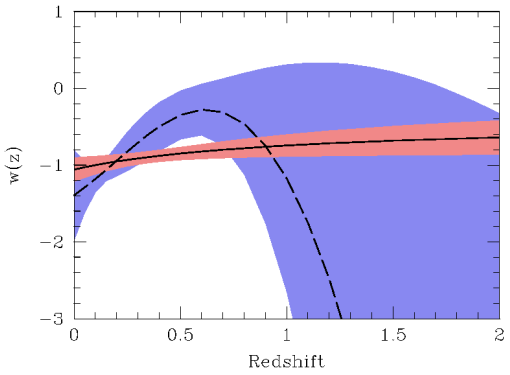
\includegraphics[width=\linewidth]{figures/chapter5/fig5.9.png}
\end{minipage}
\hfill
\begin{minipage}[c]{0.48\textwidth}
  \caption{$90\%$ confidence limits on $w(z)$ for the linear parameterisation $w(z) = w_0 + w_1 \frac{z}{1+z}$ (red) and a quartic polynomial $\sum_{i=0}^{4} w_i (\ln{}(1 + z))^{i} $ (blue) using the Gold set. The best-fit equations of state are the black lines: solid for the linear parameterisation and dashed for the polynomial.  Image credit: Fig. 10 in \cite{Riess2007}.}
  \label{fig:fig5.9}
\end{minipage}
\end{figure}


The two-dimensional models illustrate degeneracies between the different parameters. This causes difficulty if one wishes to estimate the cosmological parameters from Ia SNe alone: the data is sufficient to constrain the parameters pairwise, but insufficient to determine a value for them separately. Linear degeneracy clearly exists for the pairs $(\Omega_m , \gamma)$ (\cref{fig:fig5.4}), $(w_0 , w_1 )$ (\cref{fig:fig5.5}), whereas the other four combinations $(\Omega_m , w_0)$ (\cref{fig:fig5.2}), $(\Omega_m , w_1 )$ (\cref{fig:fig5.3}), $(w_0 , \gamma)$ (\cref{fig:fig5.6}), $(w_1 , \gamma)$ (\cref{fig:fig5.7}) display degeneracies which have a more complex curved shapes. These shapes are linear for intermediate values of the parameters, however they curve to become horizontal or vertical at either end of the credible regions.  In these locations the parameters are completely non-degenerate: a precise value for one parameter contributes no information about the value of the other. Despite this, the reduced-error and Snap sets suggest linear degeneracy may emerge from these credible regions if the distance modulus uncertainties are reduced.

The $(\Omega_m , w_0)$ credible regions replicate the results from the SNe search teams for the three observational sets. In particular \cite{Kowalski2008} confirms the discrepancy (\cref{fig:fig5.8}) I found between the Gold (\cref{fig:fig5.2}c) and Union (\cref{fig:fig5.2}b) samples. 
The $\Lambda$CDM model falls in the 1$\sigma$ region for both Constitution (\cref{fig:fig5.2}a) and Union sets, whereas it is more unlikely to be predicted from the Gold data, as it lies in the 2$\sigma$ region. The smaller-error sets have 3$\sigma$ regions which rule out the $\Lambda$CDM values and are entirely enclosed by the 1$\sigma$ regions from the respective observational sets, with the ratio of areas within 1$\sigma$ indicating a better-than-linear scaling relationship between uncertainties in $\mu(z)$ and uncertainties in the values of the cosmological parameters. The dots at the position of the $\Lambda$CDM parameter values show that only the Constitution set favour the concordance model, whereas the Union set places it at the $1-2\sigma$ boundary and the Gold set firmly in the 2$\sigma$ credible region. 
In comparison to the Constitution set, the Union set favours more negative values of the constant equation of state parameter $w_0$ for equivalent values of the fractional matter density $\Omega_m$ whereas the Gold set favours more negative $w_0$ and larger values of $\Omega_m$ . There is overlap between the 1$\sigma$ credible regions for the observational sets, however this region does not include the concordance model.

Including a time-varying equation of state 
\begin{equation*}
w(z) = \Lambda + w_1 \frac{z}{1+z} = -1 + w_1 \frac{z}{1+z}    
\end{equation*}
produces the credible regions for $(\Omega_m , w_1)$, which do not favour the $\Lambda$CDM model. 
The Constitution data (\cref{fig:fig5.4}a) places the $\Lambda$CDM parameter values at the $1 - 2\sigma$ boundary, the Gold data in the 2$\sigma$ region and the Union data at the $2-3\sigma$ region boundary, while the reduced-error sets all place $(\Omega_m , w_1) = (0.3, 0)$ outside 3$\sigma$. 
At first glance, this strongly suggests that a negative time variation in $w(z)$ is far more likely than a constant. However, this result may simply be a consequence of fixing $w_0$ at a value which does not produce a good fit to the data,\footnote{This is seen by the intersection of $w_0 = -1$ (and $w_1 = 0$ because it is fixed) with the $(\Omega_m , w_0)$ credible regions, discussed in the previous paragraph.} which causes the $w_1$ value to decrease in an attempt to improve the fit. This is supported by the degeneracy between the two parameters in the dark energy equation of state shown in the $(w_0 , w_1)$ credible regions. A model varying the fractional matter density and both equation of state parameters is necessary to gain more insight into this problem.

Next we examine the linear $(w_0 , w_1)$ correlation (Fig. ??). One may question whether this is a consequence of the equation of state constraints or truly a product of the available data. Although a flat prior was assumed for all of the parameter values, the form of the dark energy equation of state 
\begin{equation*}
    w(z) = w_0 + w_1 \frac{z}{1+z} 
\end{equation*}
acts as a strong prior, placing (perhaps unjustifiably) strong constraints on the behaviour of $w(z)$. \cref{fig:fig5.9} demonstrates this by plotting the 95\% credible region (2$\sigma$ confidence $z$ limits) on $w(z)$ for the linear parameterisation 
\begin{equation*}
    w(z) = w_0 + w_1 \frac{z}{1+z} 
\end{equation*}
(red) and a quartic polynomial 
\begin{equation*}
    w(z) = \sum_{i=0}^{4} w_i \left[ \ln(1+z) \right]^i
\end{equation*}
(blue) using the Gold set \cite{Riess2007}. The behaviour of the best-fit models for the dark energy equation of state 
differs dramatically: the linear parameterisation is (by definition) monotonically increasing as $z \rightarrow{} \infty{}$, however the quartic admits a non-monotonic evolution with recent changes (at $z < 0.1$) in $w(z)$. This suggests that the linear parameterisation generates artificially well-constrained results for w(z). Conversely, one may argue that the use of the more general equation of state is unwarranted (it merely expresses our gross ignorance, rather than being physically well-motivated,so the results may depend strongly upon the choice of prior \cite{Efstathiou2008}), as the Gold set does not have sufficient SNe (only 23 at $z > 1$) \cite{Riess2007} to place limits on such a general w(z). This problem may be resolved by using the $> 1000$ samples expected from observations with survey telescopes such as SNAP/WFIRST, the Large Synoptic Survey Telescope\footnote{LSST \url{http://www.lsst.org}} and the Panoramic Survey Telescope and Rapid Response System\footnote{Pan-STARRS \url{http://pan-starrs.ifa.hawaii.edu/public}} \cite{Leibundgut2008}. These projects will provide large, homogeneous data sets with increased numbers of SNe at z > 1, which will give tighter constraints on $w(z)$ at (relatively) high redshift \cite{Leibundgut2008}.

Finally we analyse the credible regions including interaction, for which there are no existing results from the SNe survey teams. The ($\Omega_m$ , $\gamma$) models show a linear correlation between the fractional matter density and the interaction parameter. Both the Constitution (\cref{fig:fig5.4}a) and Union (\cref{fig:fig5.4}b) sets suggest that the concordance model is plausible, since ($\Omega_m$ , $\gamma$) = (0.3, 0) lies within the 1$\sigma$ regions, however the Gold data once again disagrees, placing it only within 2$\sigma$. The Constitution 0.2x set also favours the $\Lambda$CDM model, however the Gold 0.2x and Union 0.2x sets neither agree well with $\Lambda$CDM nor their normal-error counterparts (the 1$\sigma$ regions intersect the 2 and 3$\sigma$ region of the normal-error sets). 
This is probably caused by a convergence problem with the Markov chains: both of these data–model combinations had to be run for unusually large step sizes before the resulting histogram was smooth, but they may have needed even longer before the histogram converged to the posterior. Highly negative values of $\gamma$ represent transfer of energy from matter into dark energy, resulting in $\Omega_m \rightarrow{} 0$ as $z \rightarrow{} -1$. As this result is not indicated by the observational data, these two results remain a curiosity. Overall, $\gamma$ = 0 lies within the 1$\sigma$ regions for values of $\Omega_m$ which are observationally likely, (0.25 . $\Omega_m$ . 0.5), so at this stage no interaction remains a probable result. 
The credible regions for ($w_0$ , $\gamma$) (\cref{fig:fig5.6}) and ($w_1$ , $\gamma$) (\cref{fig:fig5.7}) have degeneracies which are unlikely to be resolved. This is because the interaction in the adiabatic Friedmann equation \cref{eq:1.10} can be represented as an effective non-constant equation of state [3, 67], which contributes an additional term to w(z). As $\gamma \rightarrow{} -1$ it loses its degeneracy with $w_1$ : the credible regions (\cref{fig:fig5.7}) become horizontal, so a particular value for $\gamma$ places no constraint upon the value for $w_1$ . At the limit:

\begin{subequations}
\label{eq:5.1}
\begin{align}
    \frac{\dd{\Omega}_{m}}{\dd{z}} &=
    \frac{1}{1+z} \left(
        3 \Omega_{m} + \frac{1}{H(z)}
    \right)
    \label{eq:5.1a} \\
    \frac{\dd{\Omega}_{X}}{\dd{z}} &=
    \frac{1}{1+z} \left(
        3 \Omega_{X} \left(
            1 + w_{0} + w_{1} \frac{z}{1+z}
        \right)
        - \frac{1}{H(z)}
    \right)
    \label{eq:5.1b}
\end{align}
\end{subequations}

so in the past, as $z \rightarrow{} \infty{}$, the effect of $H(z)$ will swamp the effect of any values of $w(z)$ and the value of $\Omega_X$ will be negative,\cite{vanOsten2006} which is physically impossible (as it is a fractional density). The credible regions \cref{fig:fig5.2,fig:fig5.3,fig:fig5.4,fig:fig5.5,fig:fig5.6,fig:fig5.7} show that a large section of the 2d parameter space often lies within the 1$\sigma$ credible region, illustrating that the Friedmann equations may produce exceedingly similar distance modulus curves for very different initial conditions (fits to the data are given in §B). Therefore one must look for other observational data which does not display the same degeneracy\footnote{This statement is true only for $\Lambda$CDM-based models with a dark energy equation of state based on a barotropic model. More exotic possibilities such as the ”doomsday” and braneworld models do not display opposing degeneracies: see \cite{Rubin2008} for a summary of SN+\cmb{}+\bao{} credible regions with more exotic models.} in order to obtain tight constraints (on the order of those for the one-parameter models). 
Fortunately, the two other sources used for cosmological parameter estimation are complementary to SNe: both the \cmb{} and \bao{} display the opposite degeneracy (see \cref{sec:5.3}), at least for $\Omega_m$ , $w_0$ and $w_1$. It remains to be seen whether similar relationships exist for $\gamma$.







\section{Improving constraints: combination with CMB and BAO data}
\label{sec:5.3}

\begin{figure}
\centering
    \staticfigure{figures/chapter5/fig5.10.png}{$68.3\%$, $95.4\%$ and $99.7\%$ confidence level contours on $w_1$ (here $w_a$) and $w_0$ for a flat Universe. The Union SN set was combined with CMB or BAO constraints (left) and the SN+CMB+BAO constraints with and without the SNe systematics removed (right). The diagonal line represents $w_0 + w_a = 0$: the likelihoods based on observational data remain below it, favouring matter domination at $z \gg 1$.  Image credit: Fig. 16 in \cite{Kowalski2008}.}
\end{figure}

\begin{figure}
\centering
    \staticfigure{figures/chapter5/fig5.11.png}{Comparison of $(\Omega_M , w_0)$ credible regions from the Constitution data when two different light curve fitters are used to find the luminosity of the SNe. Left: SALT; right: MCLS2k2. Notice the shift in the position of the $\Lambda$CDM parameter values (the dot) with no change in the SNe observed, merely the data calibration. Image credit: Fig. 4 from \cite{Hicken2009}.}
\end{figure}


Tightening of cosmological parameter constraints can be achieved by combining SNe data with a range of other methods for estimating the parameters, foremost amongst which are multipoles in the power spectra from the cosmological microwave background (\cmb{}) \cite{LewisBridle2002,Spergel2007,Komatsu2010,Dunkley2009} and the correlation func- tion for luminous red galaxies from baryon acoustic oscillation (\bao{}) measurements \cite{Eisenstein2005,Carroll2001,Percival2007}. These measurements are sometimes referred to as ”standard rulers” because they directly measure fundamental cosmological distances \footnote{The ”standard candle” measures the luminosity distance because the luminosity of the object is independent of its local environment, so the ratio of the (corresponding) distance between two standard candles depends only on the intervening spatial curvature (given by the FLRW metric). Similarly, the ”standard ruler” measures the angular diameter distance because the ratios of angle subtended on the sky depends only on the spatial curvature via the FLRW metric. \cite{Hobson2006}}. 

A full estimate of the cosmological parameters from such sources requires a similar process\footnote{A summary of the \bao{} process is provided in \cite{vanOsten2006}§2.; for the \cmb{} an example of parameter extraction is \cite{LewisBridle2002} while the parameters extracted from this are summarised in \cite{vanOsten2006,Carroll2001}.} to this project: generating the relevant observational data from different values of the cosmological parameters and using a Markov chain Monte Carlo algorithm to move through the parameter space based on an acceptance/rejection scheme (e.g. Metropolis-Hastings, although much effort has been put into generating efficient schemes purely for the \cmb{} analysis \cite{Christensen2001,Dunkley2005,LewisBridle2002} ). Although credible regions for the parameters $(\Omega_m , w_0 , w_1 )$ are available from the \cmb{} \cite{Spergel2007,Komatsu2010,Dunkley2009} and $(\Omega_m , w_0)$ from \bao{} measurements \cite{Eisenstein2005,Percival2007}, they are not in a form which enabled me to compare them directly to my own results (except by sight).

A trend throughout the results has been tension between the parameter estimation produced by the Gold set and that produced by the Union and Constitution sets, which is emphasised by the lack of overlap in the credible regions for the Gold 0.2x set and the Constitution/Union 0.2x sets. This lack is easily explained if one considers the formation of the projected SNAP sets. The (unknown) parameter values for our Universe would produce a $\mu(z)$ curve according to the Friedmann equations \cref{eq:1.4}, the luminosity distance formula \cref{eq:1.15} and the theoretical distance modululs formula \cref{eq:1.13}. The $\mu(z)$ points from observations of Type Ia SNe must be calculated from the pragmatic distance modulus formula \cref{eq:1.14} once their luminosities (hence luminosity distances) are found from a light-curve fitter: the choice of corrections to obtain \cref{eq:1.13} from \cref{eq:1.14} and the choice of light curve fitter to determine \cref{eq:1.15} create a particular scatter of the data points around the \lq\lq{}true\rq\rq{} $\mu(z)$ curve. Uncertainties in these choices and limitations on the instrument precision and calibration create error bars about the data points. In this way, the jiggled Snap and Snap 0.2x sets were generated from a known set of cosmological values. The 0.2x sets for Constitution, Gold and Union have reduction in the error bars, but not in the scattering (for reasons detailed in \cref{sec:5.1}). Therefore the reduced error bars shrink the subset of parameter values which provide good fits to the data, while the same data points maintain the different scatters from the different data sets. This exaggerates the difference between the data sets, so overlap becomes more unlikely as the errors shrink. The difference between the data sets results mostly from the light curve fitters used to determine the SN luminosity: the Gold set uses the MLCS2k2 fitter \cite{Riess2007}, whereas the Union set uses the SALT fitter \cite{Kowalski2008}. The Constitution set was calibrated with four different fitters (SALT being the preferred fitter): their comparison of the effects of SALT and MLCS2k2 on the parameter estimates (\cref{fig:fig5.1a-f}) shows the same trend as my results, with the MLCS2k2 fitter placing the $\Lambda$CDM parameter values within 2$\sigma$ compared to 1$\sigma$ for SALT. The shift in credible regions increases when the SNe compared are different as well as the light-curve fitters. This illustrates the vital importance of developing new light-curve fitters which cause the credible regions from different fitters to converge. Until this task is completed, there will be uncertainties in the values of the cosmological parameters derived from SNe (see §C for more detail on this). The physical values of the parameters are obscured by our lack of knowledge of both the physical mechanisms associated with Type Ia SNe and the effect of the intervening environment \cite{Leibundgut2009}.


\section{Implications}
\label{sec:5.4}

Finding well-constrained estimates for the cosmological parameters is only one vital part of cosmology. Once the parameter values are established, one faces the task of developing physical theories which explain the parameter values. 

A particularly active field for cosmologists, quantum field theorists and particle physicists is the development of new models for dark energy, which can then be tested against the observational constraints \cite{LinderScherrer2009,Copeland2006}. The parameter values determine the density and expansion of the universe at the time of early structure formation \cite{Rees1998,Riess2009}, which will aid in developing models for the earliest astronomical objects, e.g. supermassive black holes and quasars (which may be the same thing) \cite{Rees1998}. 

In turn. this will shed light on early galaxy formation and may help solve the continuing problem of finding high-redshift objects with an age which is apparently greater than that of the Universe \cite{Krauss1997,Dunlop1996}.  Of particular concern is the need for astronomical studies to ensure that the criteria they use to judge formation models (e.g. globular cluster formation) are not cosmological-model-dependant. For example, the age of the Universe depends on the cosmological parameters (see the discussion in \cref{sec:2.4}), so this cannot be used to limit the age of early-forming objects such as globular clusters. Conversely, tight constraints on the age of the Universe (13.7 ± 0.2 Gyr for the $\Lambda$CDM model \cite{Barnes2005}) would provide an upper bound on the age of old, high-redshift objects (e.g. quasars \cite{Hasinger2002}, globular clusters \cite{Reid1998}, luminous elliptical galaxies \cite{Dunlop1996}), which would then act as a criterion for eliminating certain formation models for these objects which predicted an age older than the Universe \cite{Dunlop1996}. Beyond astronomy, the equation of state for dark energy will limit the possible physical methods by which the dark energy is generated. This impacts upon high energy physics theories which apply when the Universe is extremely young, such as supersymmetry and supergravity: see \cite{Copeland2006} for a review of this topic, which is beyond the scope of this project. Moreover, the cosmological parameter values predict the proportion of primordial light elements (H, D, He and Li) synthesized after the big bang \cite{Riess2009}, which acts as a test for dark energy represented by primordial quintessence fields \cite{Copeland2006}. The implications of a non-$\Lambda$CDM universe are present in diverse fields beyond cosmology.

In conclusion, there are currently three plausible groups of models which offer one-parameter deviations from the $\Lambda$CDM model: one favouring the Gold estimates, one favouring the Constitution/Union estimates and a compromise version that is a reasonable fit (within 1$\sigma$) for all three. The multiple- parameter models (of which only two-parameter models were examined here) have too many degeneracies to easily discern a best-fit value with 68\% confidence limits for each of the parameters. This problem may be resolved by combining the credible regions from Ia SNe with those from other data and redshift-distance relations to estimate the cosmological parameters, notably the angular diameter distance and data from the \cmb{} or \bao{}. Until the light-curve fitters which are used to reduce Type Ia SNe to standard candles are improved, the parameter estimates from different data sets (or even the same data but using different light curves) will give different credible regions for the parameters. Until then it is difficult to determine which of the families of parameter values \cref{tab:5.3} is closest to the true values for the observable Universe. Consequently, I conclude that the $\Lambda$CDM model is a reasonable approximation to the correct values which is currently unchallenged by parameter estimates derived from Type Ia SNe.
% chapters/conclusions.tex
\chapter{Conclusions}
\label{ch:conclusions}

\section{Further Work}
\label{sec:6.1}

The future work based upon this project is divided into three categories: use of the existing output as preliminary data, improvements to the current method and addition of complexity to the model, all of which may contribute to the resolution of questions posed by the current results. The first category involves the computation of the Bayes factor for each of the models. This enables a comparison of the global likelihood of two models $M_i , M_j$ which takes into account their different complexity (in this case, the number of parameters varying from the concordance model):

% Equation (6.1)
\begin{equation}
    O_{ij} 
    = \frac{ \prob{M_{i}}[I] }{ \prob{M_{j}}[I] } \frac{ \prob{D}[M_{i},I] }{ \prob{D}[M_{j},I] }
    = \frac{ \prob{M_{i}}[I] }{ \prob{M_{j}}[I] } \frac{ \mathcal{L} (M_{i}) }{ \mathcal{L} (M_{j}) }
    = \frac{ \prob{M_{i}}[I] }{ \prob{M_{j}}[I] } B_{ij}
\label{eq:bayes-factor}
\end{equation}

where the odds factor $O_{ij}$ reduces to the Bayes factor $B_{ij}$ because there is no prior reason to favour one model over the other \cite{Gregory2005}. The global likelihood of the model $M_i$ is an integral over the product of prior $\prob{x}[M_i , I]$ and likelihood $\prob{D}[x, M_i , I]$ (which is obtained as part of the calculation of the posterior):

% Equation (6.2)
\begin{equation}
    \prob{D}[M_{i},I]
    = \int{} \dd{x} \prob{x}[M_{i},I] \prob{D}[x,M_{i},I]
\label{eq:model-likelihood-integral}
\end{equation}

There are several existing methods to calculate tha Bayes factor, all of which rely either on brute-force integration or making an approximation so the the integral can be replaced by the solution of a matrix equation (e.g. the linear least-squares approximation) \cite{Gregory2005}. A new method suggested by Weinberg calculates $B_{ij}$ directly from the posteriors without the need for either method \cite{Weinberg2009}.

The second category (which will require more computing power) increases the complexity of the algorithm used to generate the Markov chains in order to achieve faster convergence to the posterior. This involves either changing the step size using parallel tempering or minimising the chain length by applying a convergence test.

The third category involves extending the complexity of the model: either introducing more parameters and/or allowing more of them to vary at once (once again, the latter will require more computing power). Of these options, the one which is most cosmologically interesting is the addition of more parameters, in particular including a more general form of the dark energy equation of state. The number of cosmological parameters which can be extrapolated from SNe data is small compared to the richness of the \cmb{} \cite{Francis2008} and the majority of additions are the inclusion of more cosmological fluids \cite{Hobson2006}:
\begin{itemize}
    \item a radiation term (dominated by the photons from the \cmb{} which is well-quantified, but also neutrinos which have the same equation of state $w = 1/3$)
    \item the separation of matter into dark and baryonic components (which would allow separate priors from different data)
    \item and a curvature term (not strictly a fluid, but it can be modelled as one) which would allow non-flat geometries.
\end{itemize}
Overall, it is likely that the addition of \cmb{} photons and a more general $w(z)$ would have the greatest impact. The latter two approaches involve repeating the project: this enables the inclusion of the most up to date SNe data (currently \cite{Amanullah2010}, or this may include active observing for Ia SNe and reanalysis of the ”global” SNe data using new light curves). The method from this project (or some improved variant) can also be repeated with data from other sources, notably \cmb{}, \bao{} and constraints from nucleosynthesis. The future work for this project is particularly rich, encompassing numerical, theoretical and observational fields.

\section{Summary}
\label{sec:6.2}

Distance-redshift relations are sensitive to the values of the cosmmological parameters both locally and at high redshift. Distance modulus data obtained from three recent Type Ia SNe surveys was used as a comparative tool to evaluate the consistency of various cosmological models. Five additional SNe sets were artificially generated: three examining how the error in the cosmological parameters scales with reduction of errors from the SNe data and two providing projected results from a newly- proposed space-based survey. The aim of the project was to determine best-fit values and confidence limits for the cosmological parameters across all data sets by application of Bayesian inference, using Markov chain Monte Carlo methods to determine the posteriors from which these values were extracted.

During the course of the project, I demonstrated the following:

\begin{itemize}
\item On large scales, the contents of the Universe are well-approximated by a series of cosmological fluids with various equations of state. If the energy pressure of a fluid is negative, then it falls into a class of fluids known as dark energy.
\item The Friedmann-Lemaitre-Robertson-Walker metric which determines the evolution of the Universe follows directly from the application of the cosmological principle (homogeneity and isotropy) to the field equations of general relativity.
 \item The Friedmann equations are a set of numerically integrable, coupled, first-order ODEs which arise from the FLRW metric and the requirement of local energy conservation. The diagonal form of the metric permits only perfect fluids to be included in the Friedmann equations.
\item This restriction narrows the classes of dark energy which could be examined by this project. In particular it eliminates quintessence fields while still permitting barotropic fluids and a cosmological constant.
\item The luminosity distance-redshift relation is a robust method for estimating values of the cosmological parameters using suitably calibrated Type Ia supernovae as standard candles.
\item Cosmological parameter estimation can be achieved by application of Bayesian inference, which generates a posterior probability density function (PDF) taking into account prior information and observational data.
\item Calculation of the posterior PDF can be achieved numerically with reasonable efficiency using Markov chain Monte Carlo methods, the simplest of which is the Metropolis-Hastings algorithm. The simplicity of this algorithm means that some fine-tuning is required before convergence to the posterior is achieved.
\item The one- and two-parameter posteriors can be converted into credible regions which summarise the probability that a subset of parameter values contains the values corresponding to the observable Universe.
\item Analysis of the one-parameter results demonstrates that the 1d parameter values agree with the concordance model if all data sets are taken into account. Individual data sets show better fits to non-concordance values, however the tension between the Gold set and the Constitution and Union sets results in no single non-concordance values being a good fit to all three SNe sets. 
\item This tension increases when one scales the errors on the observed data sets, demonstrating the difference in light curve calibration between the Gold set and the Constitution/Union sets. When these smaller-error sets are compared to the projected SNAP sets, the uncertainty in the best-fit cosmological parameters is comparable to the uncertainty from the estimated ”pessimistic” result from the proposed SNAP/WFIRST survey. The optimistically estimated result has uncertainties which are superior to current results by up to an order of magnitude.
\item The two-parameter models show degeneracy between parameters, which increases the difficulty in constraining parameter values. Current observation have phase space regions of linear degeneracy between all parameters. Excluding the $(\Omega_m , \gamma)$ and $(w_0 , w_1)$ models, these credible regions curve into areas of non-degeneracy, inside of which a value of one parameter provides no constraints on the others. Examination of the corresponding regions for the artificially generated sets suggests that linear degeneracy will emerge for all of the two-parameter models if the errors in the data are reduced. 
\item Until improved light-curve fitters (\cref{app:type-ia-standard-candles}) are developed, values of the cosmological parameters derived from Type Ia SNe will be highly sensitive to the fitters used. This accounts for the overwhelming majority of the tension between the Gold set and the Constitution/Union sets.
\item These degeneracies force us to obtain data with complementary degeneracies in order to tightly constrain the parameters. This is currently available for a three-parameter space $(\Omega_m , w_0 , w_1 )$ from the seven-year WMAP data from the cosmic microwave background and Sloan Digital Sky Survey data on baryon acoustic oscillations.
\end{itemize}


\appendix

% chapters/appendixA.tex
\chapter{Large figures from results}
\label{app:large-figures}

This chapter is designed to be viewed in conjunction with the Results section \cref{ch:results}. It contains enlarged versions of the posterior PDFs for each parameter in the single-parameter models (not marginalised over $H_0$ ). Each data set is denoted by a different colour, with the $1\sigma$ credible region in the lightest shade and $3\sigma$ the darkest. Regions in black are outside $3\sigma$. The mean and the range of the $1\sigma$ region are shown above the posteriors by a dot and horizontal error bars. The figures show:
\begin{enumerate}
\renewcommand{\labelenumi}{(\alph{enumi})}
    \item the Hubble parameter $h/h_{72}$
    \item the matter density $\Omega_m$
    \item the constant equation of state parameter $w_0$
    \item the varying equation of state parameter $w_1$; and
    \item the mixing factor $\gamma$.
\end{enumerate}

\staticfigure[0.8\textwidth]
  {figures/appendixA/figA1a.png}
  {Posterior for the Hubble parameter $h/h_{72}$.}

\staticfigure[0.8\textwidth]
  {figures/appendixA/figA1b.png}
  {Posterior for the matter density $\Omega_M$.}

\staticfigure[0.8\textwidth]
  {figures/appendixA/figA1c.png}
  {Posterior for the constant equation of state parameter $w_0$.}

\staticfigure[0.8\textwidth]
  {figures/appendixA/figA1d.png}
  {Posterior for the varying equation of state parameter $w_1$.}

\staticfigure[0.8\textwidth]
  {figures/appendixA/figA1e.png}
  {Posterior for the mixing factor $\gamma$.}

% chapters/appendixB.tex
\chapter{Comparison of distance modulus curves to data}
\label{app:distance-modulus-curves}

The following plots show the $\mu(z)$ curves for each dataset and single-parameter model overlaid on the SNe data. The curves were generated using the Friedmann equation solver, with the initial condition corresponding to the single-parameter model: the concordance model ($\Lambda$CDM) with the $H_0$ value changed to that assumed by the SNe teams and the free parameter changed to the best-fit value from the corresponding posterior. The curves formed with the free parameter at 68\% confidence limits and the $\Lambda$CDM value are also plotted for comparison. 

Unfortunately, as $\mu(z)$ is a logarithmic measure of the luminosity distance, variations in the cosmological parameters do not necessarily create differences in $\mu(z)$ which are easily discernible by eye. This is particularly evident in the plots for the SNAP set, in which the $\Lambda$CDM model and the parameter values are identical to within one part in $10^{-2}$. Moreover, the parameters at 68\% CL produce distance modulus curves which are close to each other and that of the $\Lambda$CDM curve. Therefore the dotted lines were used for the 68\% parameter curves to (hopefully) show the plotting of one over the other.

\clearpage

\section{Constitution set}
\label{sec:constitution-set}

\staticfigure[0.75\textwidth]
  {figures/appendixB/figB1a.png}
  {Distance modulus curves for the Constitution set with varying $\Omega_M$.}

\staticfigure[0.75\textwidth]
  {figures/appendixB/figB1b.png}
  {Distance modulus curves for the Constitution set with varying $w_0$.}

\staticfigure[0.75\textwidth]
  {figures/appendixB/figB1c.png}
  {Distance modulus curves for the Constitution set with varying $w_1$.}

\staticfigure[0.75\textwidth]
  {figures/appendixB/figB1d.png}
  {Distance modulus curves for the Constitution set with varying $\gamma$.}

\section{Constitution 0.2x set}
\label{sec:constitution-02x-set}

\staticfigure[0.75\textwidth]
  {figures/appendixB/figB2a.png}
  {Distance modulus curves for the Constitution 0.2x set with varying $\Omega_M$.}

\staticfigure[0.75\textwidth]
  {figures/appendixB/figB2b.png}
  {Distance modulus curves for the Constitution 0.2x set with varying $w_0$.}

\staticfigure[0.75\textwidth]
  {figures/appendixB/figB2c.png}
  {Distance modulus curves for the Constitution 0.2x set with varying $w_1$.}

\staticfigure[0.75\textwidth]
  {figures/appendixB/figB2d.png}
  {Distance modulus curves for the Constitution 0.2x set with varying $\gamma$.}


\section{Gold set}
\label{sec:gold-set}

\staticfigure[0.75\textwidth]
  {figures/appendixB/figB3a.png}
  {Distance modulus curves for the Gold set with varying $\Omega_M$.}

\staticfigure[0.75\textwidth]
  {figures/appendixB/figB3b.png}
  {Distance modulus curves for the Gold set with varying $w_0$.}

\staticfigure[0.75\textwidth]
  {figures/appendixB/figB3c.png}
  {Distance modulus curves for the Gold set with varying $w_1$.}

\staticfigure[0.75\textwidth]
  {figures/appendixB/figB3d.png}
  {Distance modulus curves for the Gold set with varying $\gamma$.}
 
\section{Gold 0.2x set}
\label{sec:gold-02x-set}

\staticfigure[0.75\textwidth]
  {figures/appendixB/figB4a.png}
  {Distance modulus curves for the Gold 0.2x set with varying $\Omega_M$.}

\staticfigure[0.75\textwidth]
  {figures/appendixB/figB4b.png}
  {Distance modulus curves for the Gold 0.2x set with varying $w_0$.}

\staticfigure[0.75\textwidth]
  {figures/appendixB/figB4c.png}
  {Distance modulus curves for the Gold 0.2x set with varying $w_1$.}

\staticfigure[0.75\textwidth]
  {figures/appendixB/figB4d.png}
  {Distance modulus curves for the Gold 0.2x set with varying $\gamma$.}

\section{Union set}
\label{sec:union-set}

\staticfigure[0.75\textwidth]
  {figures/appendixB/figB5a.png}
  {Distance modulus curves for the Union set with varying $\Omega_M$.}

\staticfigure[0.75\textwidth]
  {figures/appendixB/figB5b.png}
  {Distance modulus curves for the Union set with varying $w_0$.}

\staticfigure[0.75\textwidth]
  {figures/appendixB/figB5c.png}
  {Distance modulus curves for the Union set with varying $w_1$.}

\staticfigure[0.75\textwidth]
  {figures/appendixB/figB5d.png}
  {Distance modulus curves for the Union set with varying $\gamma$.}

\section{Union 0.2x set}
\label{sec:union-02x-set}

\staticfigure[0.75\textwidth]
  {figures/appendixB/figB6a.png}
  {Distance modulus curves for the Union 0.2x set with varying $\Omega_M$.}

\staticfigure[0.75\textwidth]
  {figures/appendixB/figB6b.png}
  {Distance modulus curves for the Union 0.2x set with varying $w_0$.}

\staticfigure[0.75\textwidth]
  {figures/appendixB/figB6c.png}
  {Distance modulus curves for the Union 0.2x set with varying $w_1$.}

\staticfigure[0.75\textwidth]
  {figures/appendixB/figB6d.png}
  {Distance modulus curves for the Union 0.2x set with varying $\gamma$.}

\section{SNAP set}
\label{sec:snap-set}

\staticfigure[0.75\textwidth]
  {figures/appendixB/figB7a.png}
  {Distance modulus curves for the \textsc{snap} set with varying $\Omega_M$.}

\staticfigure[0.75\textwidth]
  {figures/appendixB/figB7b.png}
  {Distance modulus curves for the \textsc{snap} set with varying $w_0$.}

\staticfigure[0.75\textwidth]
  {figures/appendixB/figB7c.png}
  {Distance modulus curves for the \textsc{snap} set with varying $w_1$.}

\staticfigure[0.75\textwidth]
  {figures/appendixB/figB7d.png}
  {Distance modulus curves for the \textsc{snap} set with varying $\gamma$.}

\section{SNAP 0.2x set}
\label{sec:snap-02x-set}

\staticfigure[0.75\textwidth]
  {figures/appendixB/figB8a.png}
  {Distance modulus curves for the \textsc{snap} 0.2x set with varying $\Omega_M$.}

\staticfigure[0.75\textwidth]
  {figures/appendixB/figB8b.png}
  {Distance modulus curves for the \textsc{snap} 0.2x set with varying $w_0$.}

\staticfigure[0.75\textwidth]
  {figures/appendixB/figB8c.png}
  {Distance modulus curves for the \textsc{snap} 0.2x set with varying $w_1$.}

\staticfigure[0.75\textwidth]
  {figures/appendixB/figB8d.png}
  {Distance modulus curves for the \textsc{snap} 0.2x set with varying $\gamma$.}

% chapters/appendixC.tex
\chapter{Are Type Ia SNe standard candles?}
\label{app:type-ia-standard-candles}

% ---------- Appendix C ----------

\begin{table}
\centering
\begin{threeparttable}
\caption{Characteristics of the photometric passbands used in supernova observations.}
\label{tab:C.1}

\begin{tabular}{ccc}
\toprule
Band &
Effective central wavelength (nm) &
FWHM range (nm) \\
\midrule
B & 445 & 94 \\
V & 551 & 88 \\
R & 658 & 138 \\
I & 806 & 149 \\
\bottomrule
\end{tabular}

\begin{tablenotes}
\small
\item The wavelengths cover three visible bands (B, V and R) and one near-infrared band (I).
\end{tablenotes}

\end{threeparttable}
\end{table}
```


\begin{figure}
    \centering
\staticfigure
    {figures/appendixC/figC.1.png}
    {Sample light curves for SNe, showing the relationship between various key parameters in the light-curve fitting equations. Image credit: Slide from \cite{Lidman2010b}.}
\end{figure}

\begin{figure}
\staticfigure
    {figures/appendixC/figC.2.png}
    {Comparison of the credible regions in two-parameter cosmological models using the SALT and MLCS2k2 light-curve fitters. ``Union+CfA3'' refers to the Constitution set. ``Old'' refers to the Essence set, which has better systematics and is roughly equivalent to the Union set without approximately 100 high-$z$ SNe. Image credit: Fig.~4 in \cite{Hicken2009}.}
\end{figure}

\begin{figure}
\staticfigure
    {figures/appendixC/figC.3.png}
    {Dependence of SN brightness on the star formation rate of the host galaxy. Galaxies contain SNe with greater brightness contribution from the colour parameter if they have low star-formation rates. Image credit: Slide 37 from \cite{Lidman2010b}.}
\end{figure}

\begin{figure}
\staticfigure
    {figures/appendixC/figC.4.png}
    {Dependence of SN brightness on the metallicity of the host galaxy. Metal-rich galaxies contain brighter SNe at peak brightness in the B-band than metal-poor galaxies. Image credit: Slide 40 from \cite{Lidman2010b}.}
\end{figure}

\begin{figure}
\staticfigure
    {figures/appendixC/figC.5.png}
    {Dependence of the deviation from the mean peak absolute magnitude at different observing wavelengths. The H-band in the infrared has the smallest range within the SNe sample. Image credit: Slide 47 from \cite{Lidman2010b}.}
\end{figure}

The dependence of cosmological parameter estimation on the methods used to reduce Type Ia SNe to standard candles becomes increasingly important as the global set of SNe data expands. This chapter outlines the data processing and calibration undertaken by the SNe survey teams, with particular emphasis on the light curve fitting techniques used and how the field has improved since the release of each data set.

\section{Supernova photometry}
\label{sec:C.1}

Typical processes for supernova data collection are given in \cite{Kowalski2008,Hicken2009,Guy2005,Rubin2008}. 
Large-scale surveys use wide-field ($\sim 1$ square degree) CCD cameras to collect repeated images of (preferably low-extinction) fields of the sky over several months \cite{Riess2007}. Camera filters at different wavelength ranges (detailed in \cref{tab:C.1}) allow multi-colour light curves to be found for SN near \lq\lq{}maximum light\rq\rq{} (i.e. the SN at peak brightness), which are required for photometric calibration \cite{Lidman2010b}. 
The data are sent through two or more computer pipelines which subtract the new images from (older) reference images, removing the background \cite{Guy2010}. 
This leaves only the changes between the two images, enabling the generation of lists of possible SN candidates (since SN are by definition transient objects) \cite{Leibundgut2008}. The candidates are checked against a database of existing variable objects (e.g. variable starts, active galactic nuclei) and visually inspected to select the SN \cite{Guy2010}. 
Spectroscopic follow-up is allows the classification of the SN into different types shown in \cref{fig:fig1.2} and identification of their redshifts using a computer algorithm \cite{Riess2007}. Only once accurate photometry and secure classification are achieved can the Type Ia SNe be used as distance indicators \cite{Leibundgut2009}.

The practical relation between SNe observables and luminosity distance is \cref{eq:1.14}:

\begin{equation}
    m(z) - M
    = 5 \log h + 42.38 + \kappa(z) + A(z) + 5 \log D_{L}(z)
\label{eq:sn-distance-modulus}
\end{equation}

so the distance $D_L$ can only be found after the peak apparent magnitude $m(z)$ is known from observations, corrections are made for the absorption factor $A(z)$ and the $k$-correction $\kappa(z)$ and the peak absolute magnitude $M$ is found from the light curve fitters. 
The first step in this process is $k$-correction: adjusting for the fact that the data at different redshifts is compared to standards at different rest-frame wavelengths \cite{Hogg2002}. 
Absorption of the light by the interstellar medium and correction for time dilation are made using an empirical formula for $A(z)$ \cite{Blondin2008}. Part of this correction is related to extinction: the decrease in brightness (hence increase in magnitude) due to reddening and absorption of light by the interstellar medium \cite{Hogg2002}. 
The next stage in the process is the use of a photometric light curve fitter to estimate the peak absolute magnitude of the Ia SNe from the properties of the light curve and the apparent magnitude \cite{Lidman2010b}. The light curves obey a \lq\lq{}bluer-broader-brighter\rq\rq{} relation \cref{fig:figC.1} by which the spread in their intrinsic luminosities is reduced \cite{Hicken2009}. The empirical relation which is used to relate these parameters to the apparent magnitude is called a light-curve fitter \cite{Guy2005}. A number of different fitters have been developed, but the important ones are those used to reduce the Gold sample — MCLS2k2 — and the Union sample — SALT. Both of these fitters are used on the Constitution set.

\section{The SALT Fitter}
\label{sec:C.2}

The Spectral Adaptive Light Curve Template SALT is a phenomenological model for determining Ia SN light curves \cite{Guy2005}. The model was constructed from a minimal set of parameters: stretch $s$, colour $c$, and rest-frame peak magnitude in the B-band $m_{B}^{\mathrm{max}}$ (from the flux normalisation).\footnote{An additional parameter, the time of maximum light in the B-band $t$, turns out to be a nuisance parameter when the program is used for cosmological fits \cite{Guy2005}.} These parameters are inserted into the model with coefficients $\alpha$ and $\beta$:

\begin{equation}
    \mu_{B}
    = m_{B}^{\mathrm{max}} - M_{B}
    + \alpha(s-1)
    - \beta c
\label{eq:salt-distance-modulus}
\end{equation}

where $\mu_B$ is the desired distance modulus and $M$ is the absolute magnitude \cite{Hicken2009}. The coefficient values are determined by training the fitter using existing data and an iterative algorithm \cite{Guy2005}:

\begin{itemize}
    \item Start with a correction function $K = 0$
    \item Fit light curves from the data using the current K.
    \item Find the light curve residuals and propose an additional adjustment $\delta{}K$ accordingly.
    \item Update: $K \rightarrow{} K + \delta{}K$
    \item Finish when $\delta{}K$ becomes negligible.
\end{itemize}

Therefore before the fitter is used, one requires an existing set of nearby and distant SNe to be used for training and a second set which acts as a test sample for consistency checks \cite{Guy2005}. Once the coefficients are determined and verified, the template fitter can be used to determine distances. Unlike the MCLS2k2 fitter, the SALT fitter accounts for the k-correction and absorption within the fitter, so the data does not need to be adjusted before fitting. This illustrates a potential weakness of the SALT method: the intrinsic colour of the light curve is not distinguished from the host reddening due to redshift and the local environment of the SNe \cite{Hicken2009}. Therefore both low-z and high-z SNe must have the same combined (host+intrinsic) colour-magnitude relations. Since the treatment of host reddening is the largest contributor to systematic uncertainties in the luminosity distance-redshift relation (therefore also in the cosmological parameter estimation), this effectively signs the death warrant for the use of SALT on future surveys \cite{Leibundgut2008}.

\section{The MLCS2k2 Fitter}
\label{sec:C.3}

The updated Multicolour Light Curve Shape method MCLS2k2 is a template-based method similar to SALT \cite{Jha2007}. Different parameters are employed: a shape/luminosity parameter $\Delta{}$, host-galaxy extinction $A_V$ , a reddening parameter $R_V$ and the time of maximum light in the B-band $t$ \cite{Jha2007}. 
Consequently, explicit estimates of the host reddening contribution to the light curve can be made by determining $A_V$ from a prior on the difference in extinction at the $B$ and $V$ wavelengths and a chosen value for $R_V$. This is a key difference between the MCLS2k2 and the SALT method \cite{Hicken2009}. 
Like SALT, this method also employs a training algorithm and consistency checks using a test set of SNe. The particular weakness of this fitter is the uncertain value for the constant $R_V$: the developers of this technique suggest $R_V = 2.7$ but admit that the constraints that can be placed on this parameter from optical observations are weak. 
In order to test the sensitivity of the cosmological parameter estimates to the value of $R_V$, \cite{Hicken2009} used the MCLS2k2 fitter with two values: 1.7 and 3.1 and found that the larger value underestimates the distance modulus (by over-correcting for extinction) however the smaller value produces plausible results. Riess et al. used $R_V$ = 1.7 to calibrate the Gold set \cite{Riess2007}.

\section{Are the fitting parameters universal?}
\label{sec:C.4}

The three fitting coefficients $\alpha$, $\beta$ and MB for SALT and their relations in MCLS2k2 may be constant for all Ia SNe or they may change with redshift \cite{Lidman2010b}. 
Of particular concern are evolutionary trends and population differences: this reduces the homogeneity of the survey samples and increases the complexity of the light curve fitters \cite{Lidman2010b}. For example \cite{Lampeitl2010} find that \lq\lq{}passive\rq\rq{} galaxies with low star formation rates contain Ia SNe which are $0.1 - 0.04$ magnitudes brighter ($2\sigma$ or 95\%CL) at maximum light than their counterparts in host galaxies undergoing active star formation \cref{fig:figC.3}. 
This is due to a different best-fit gradient for the colour parameter $c$, i.e. $\beta$ depends on the star-formation rate of the host galaxy \cite{Lidman2010b}. They suggest a correction parameter based upon the mass of the host galaxy \cite{Lampeitl2010}. 
Moreover, the SNe in star-forming galaxies are best fit to the MCLS2k2 fitter with $R_V \sim 2$ whereas those in passive galaxies are better fit with $R_V \sim 1$ \cite{Lampeitl2010}. 
This poses a particular weakness of the MCLS2k2 fitter when used for cosmological surveys, as only one value of $R_V$ can be used across the entire data set \cite{Hicken2009}.

The absolute magnitude at peak brightness in the B-band, $M_B$ depends on the metallicity of the host galaxy \cref{fig:figC.4}. Nearby SNe are located in metal-rich galaxies, while high-$z$ SNe are in metal-poor galaxies, as these have had fewer cycles of star formation releasing metals into the interstellar medium. Thus we can conclude that $M_B$ is not a universal parameter, but is redshift-dependant \cite{Lidman2010b}. 
There is currently no evidence that the stretch coefficient $\alpha$ is environment-dependant \cite{Linder2009}. 
Therefore, while we conclude that $\alpha$ is a universal parameter, $\beta$ and $M_B$ are not. This is problematic for SNe surveys wishing to reduce large numbers of SNe with the same light curve fitter unless more complex fitters are introduced which account for these dependencies.

\section{Future developments}
\label{sec:C.5}

The key to improvements in the light-curve fitters is increased understanding of both the physical mechanisms of Type Ia SNe and the morphology of their environment \cite{Leibundgut2008}. A possible resolution to the scattering in MB is to measure the light curves in the infra-red \cite{Leibundgut2008} where the deviation from the mean is reduced \cref{fig:figC.5}. Recent research by \cite{Maeda2010} suggests that asymmetry in the thermonuclear explosion mechanism which causes a Type Ia SNe may account for the spectral diversity, however the computation requirements for the modelling are intensive and following up their results is a non-trivial task. 

The cosmological parameter estimates from the three SNe survey groups \cref{tab:5.2} show that the statistical uncertainties have reached the level of systematic uncertainties, so simply increasing the sample size of the SNe sets will not improve on the parameter constraints. Instead progress must be made on more detailed understanding of the various astrophysical effects which cause Type Ia SNe to deviate from the behaviour of perfect standard candles \cite{Leibundgut2008}. 
The physical nature of the light curve shape is crucial to the extraction of accurate distance modulus data from the observations. Accordingly, our knowledge of the intrinsic colour variations in Type Ia SNe, the influence of dust absorption in the intervening interstellar medium, demographic shifts according to the host galaxy properties and evolutionary trends as a function of redshift must be improved if we are to make further progress at estimating the cosmological parameters.


\printbibliography

\end{document}
